\chapter{Prezentarea aplica\c tiei}

Acest capitol parcurge aplica\c tia a\c sa cum o vede un utilizator real, de
la prima pagin\u a p\^ an\u a la modulul de analiz\u a. Pentru fiecare ecran am
inclus o captur\u a din versiunea func\c tional\u a, \^ inso\c tit\u a de o scurt\u a
descriere a rolului s\u au \c si a modului de utilizare. Toate capturile provin
din aplica\c tia rulat\u a local, cu date reale de antrenament.

\section{Pagina de start (Landing Page)}

Prima pagin\u a pe care o vede un vizitator neautentificat este prezentat\u a
\^ in figura~\ref{fig:landing}. Aceasta explic\u a pe scurt ce face aplica\c tia
\c si ofer\u a butoanele de autentificare \c si \^ inregistrare. Am p\u astrat-o
deliberat simpl\u a \c si direct\u a -- scopul ei este doar s\u a conduc\u a
vizitatorul c\u atre crearea unui cont.

\begin{figure}[H]
  \centering
  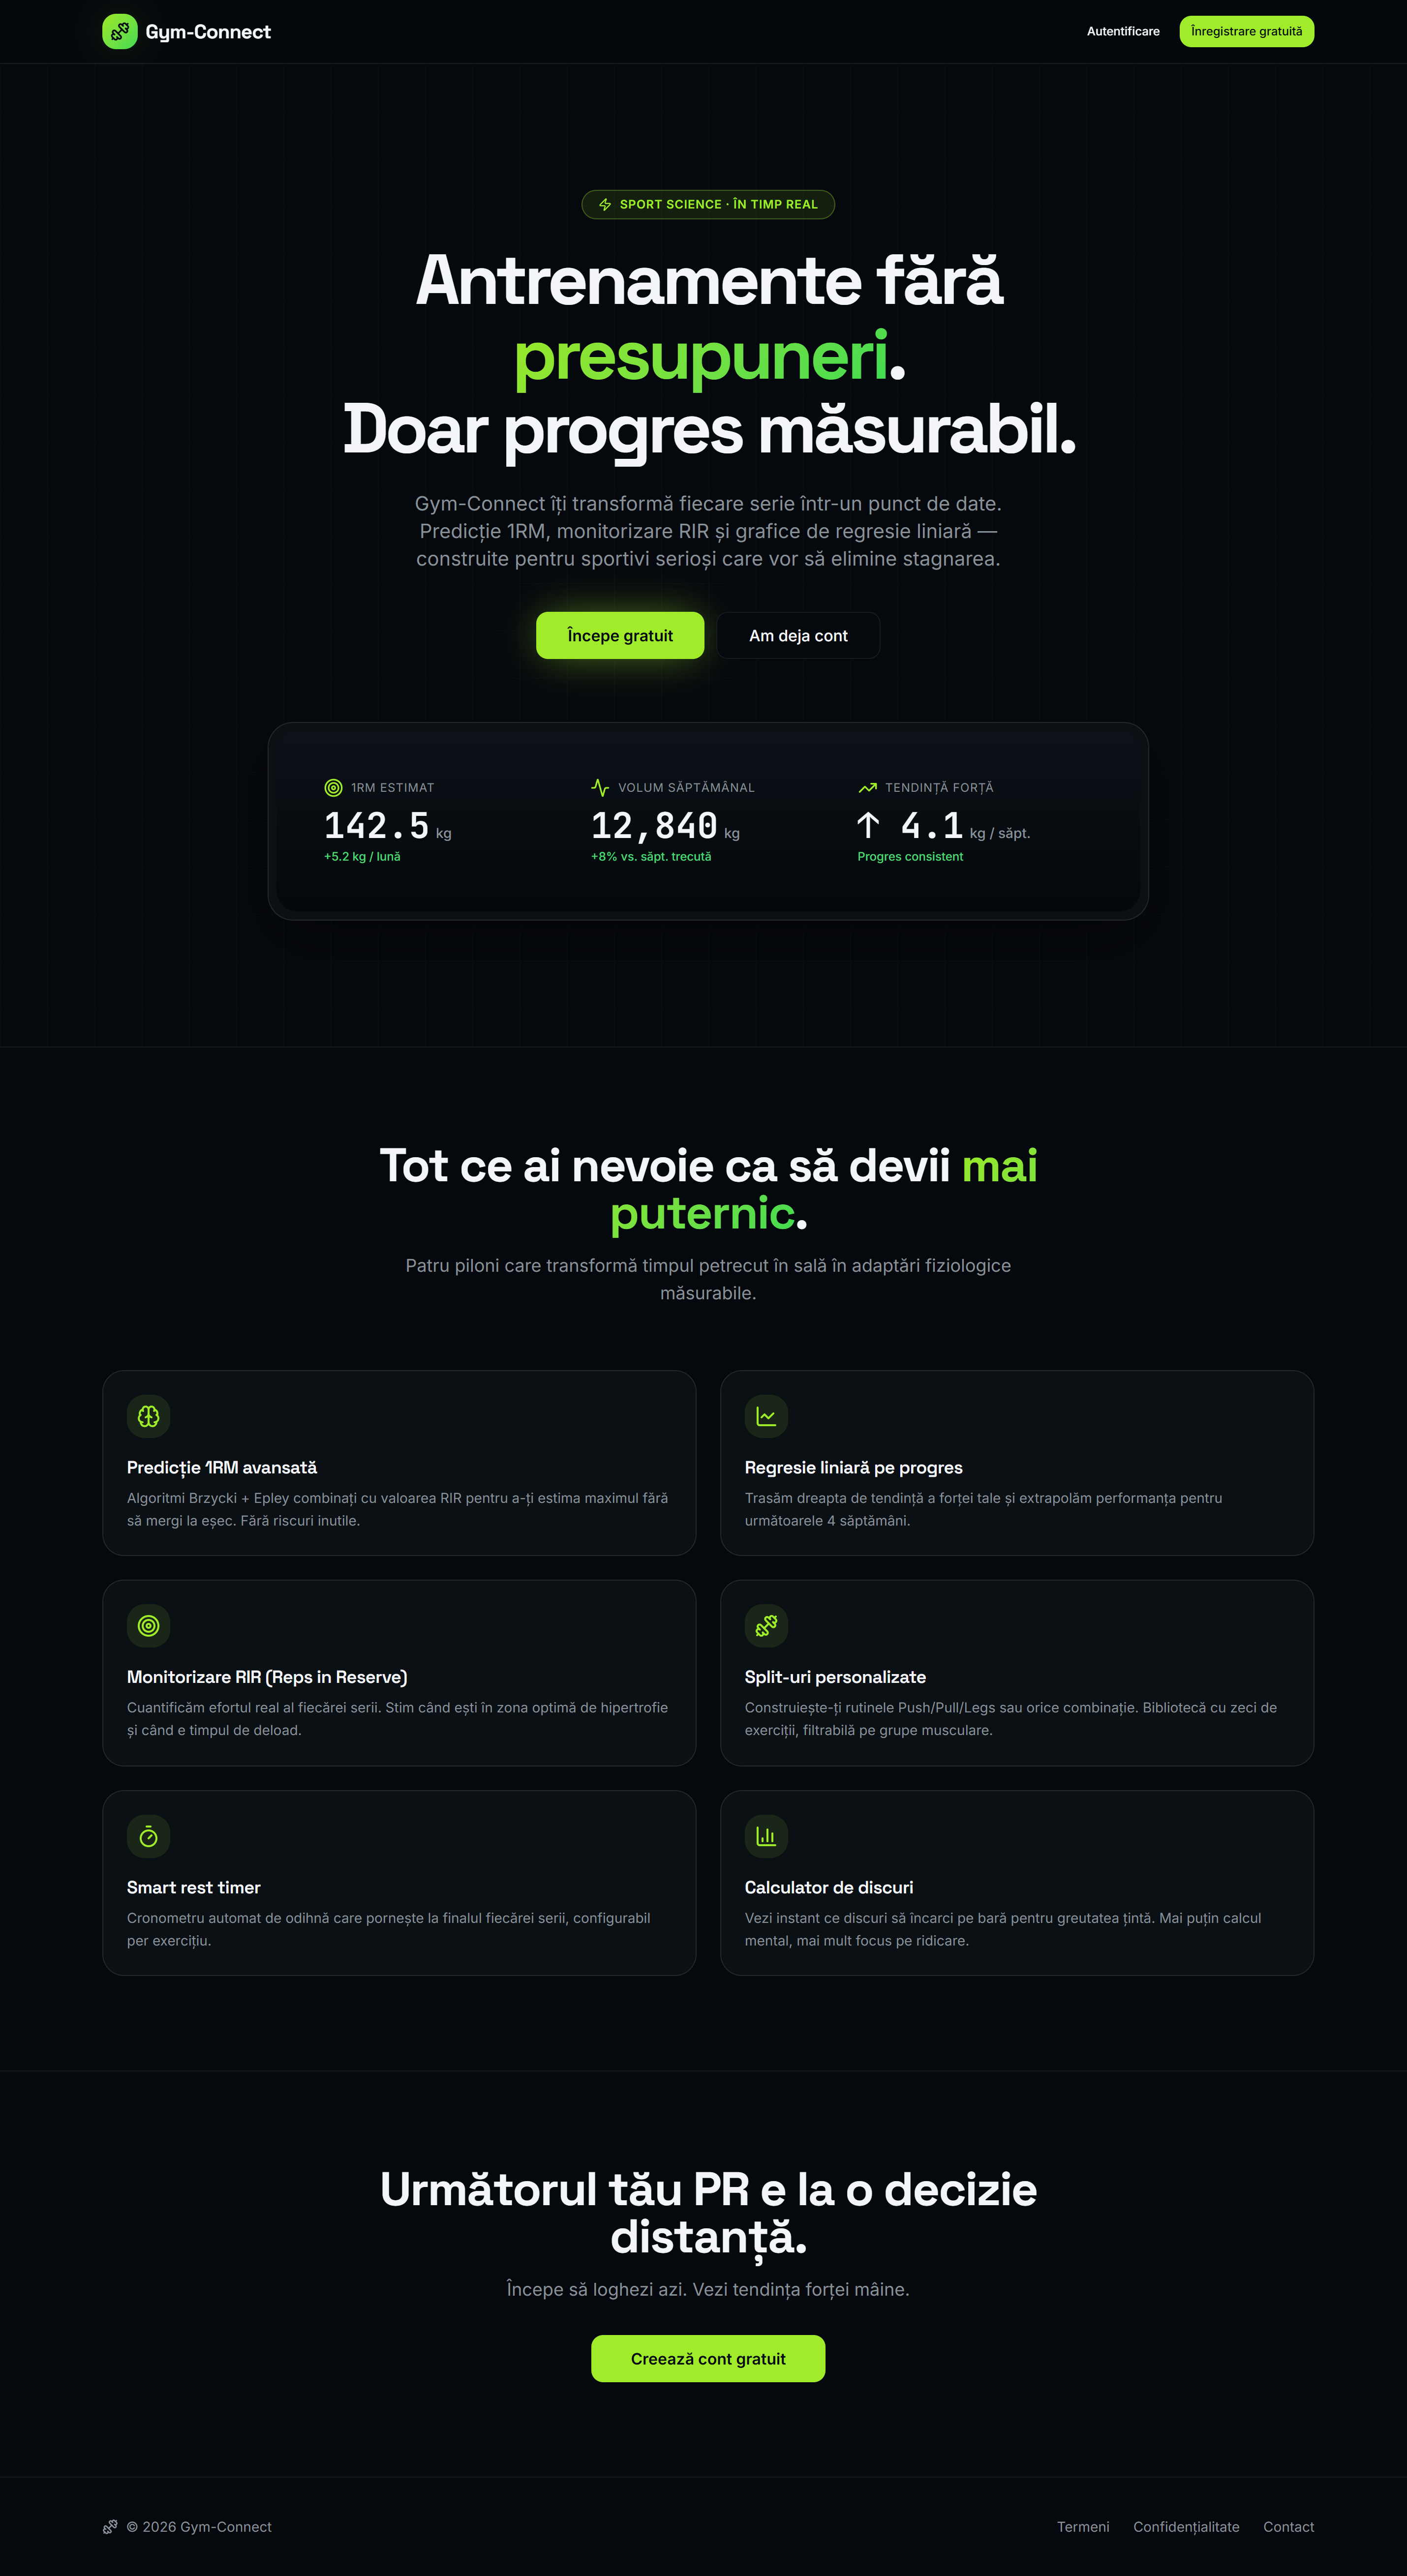
\includegraphics[height=0.78\textheight]{landing.png}
  \caption{Pagina de start (Landing Page)}
  \label{fig:landing}
\end{figure}

\section{Autentificare \c si \^ inregistrare}

Autentificarea \c si \^ inregistrarea sunt gestionate integral de Clerk, prin
componentele sale predefinite. Figura~\ref{fig:login} prezint\u a pagina de
autentificare, unde utilizatorul \^ i\c si introduce email-ul \c si parola sau
folose\c ste un cont social. Toat\u a logica sensibil\u a -- validarea parolei
\c si gestionarea sesiunii -- r\u am\^ ane \^ in sarcina Clerk.

\begin{figure}[H]
  \centering
  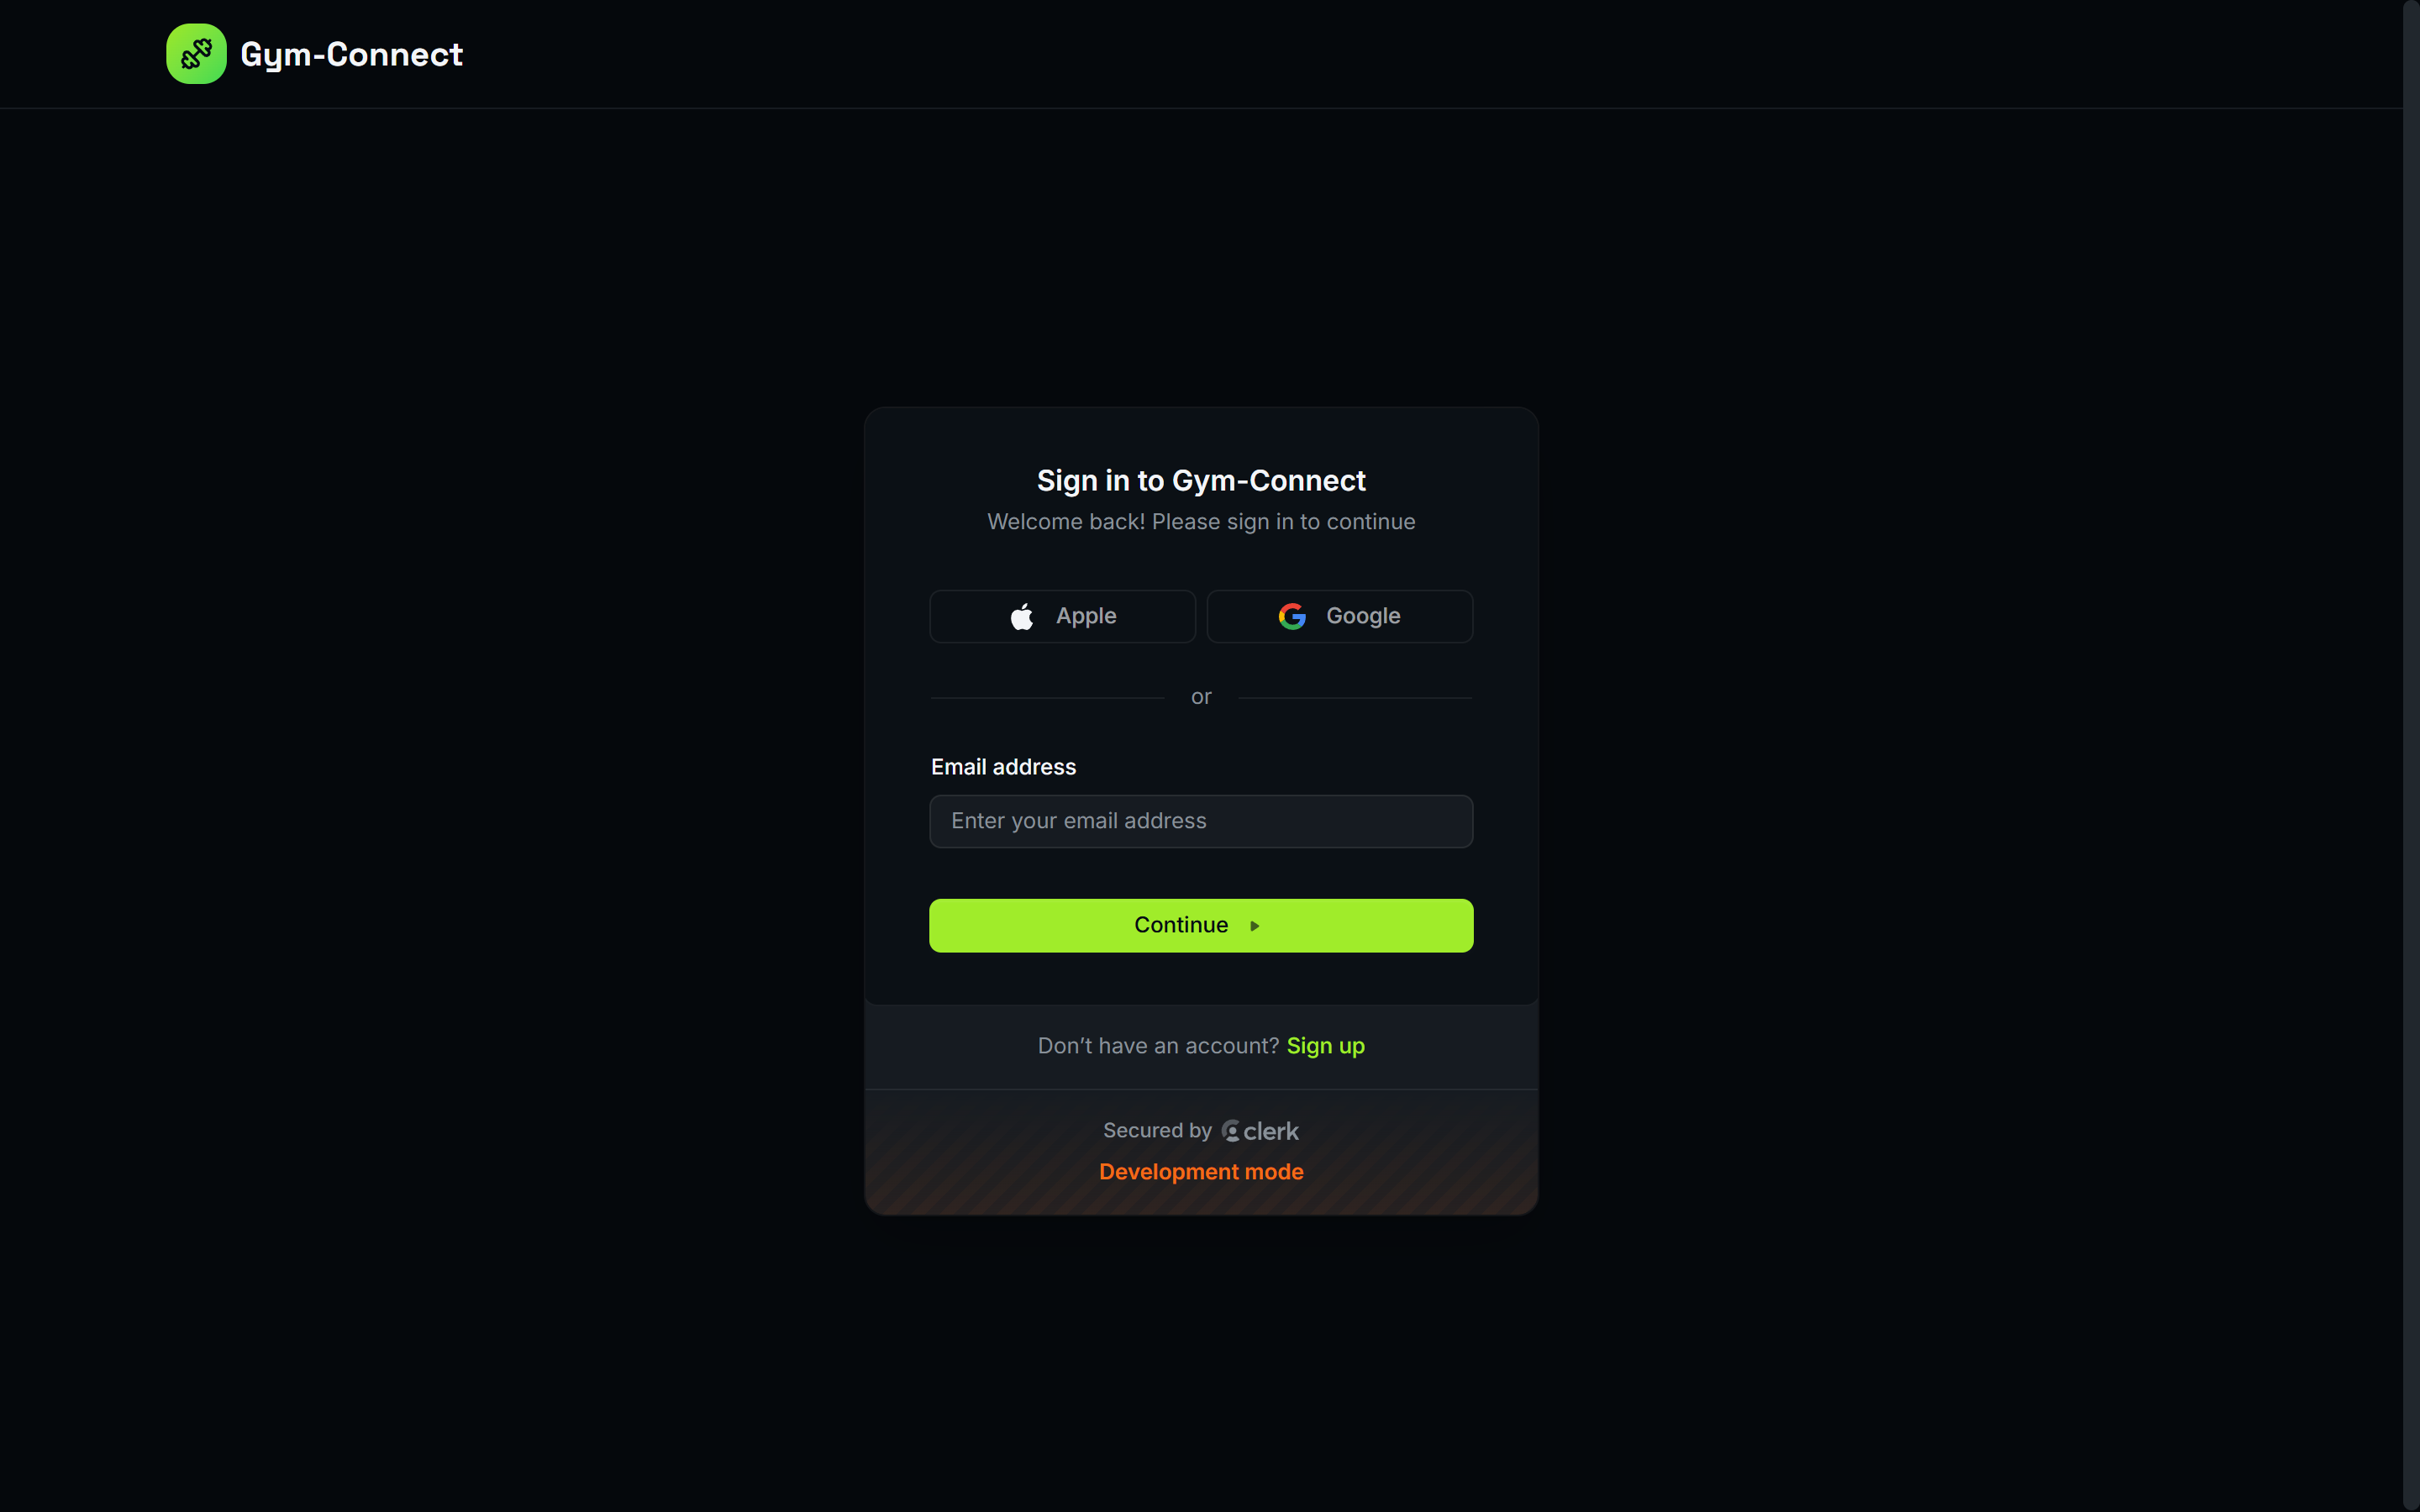
\includegraphics[width=\textwidth]{login.png}
  \caption{Pagina de autentificare}
  \label{fig:login}
\end{figure}

Pagina de \^ inregistrare, ilustrat\u a \^ in figura~\ref{fig:register}, urmeaz\u a
acela\c si tipar. Un utilizator nou \^ i\c si creeaz\u a contul \^ in c\^ ateva
secunde, iar din acel moment toate datele lui de antrenament vor fi legate de
identificatorul unic primit de la Clerk.

\begin{figure}[H]
  \centering
  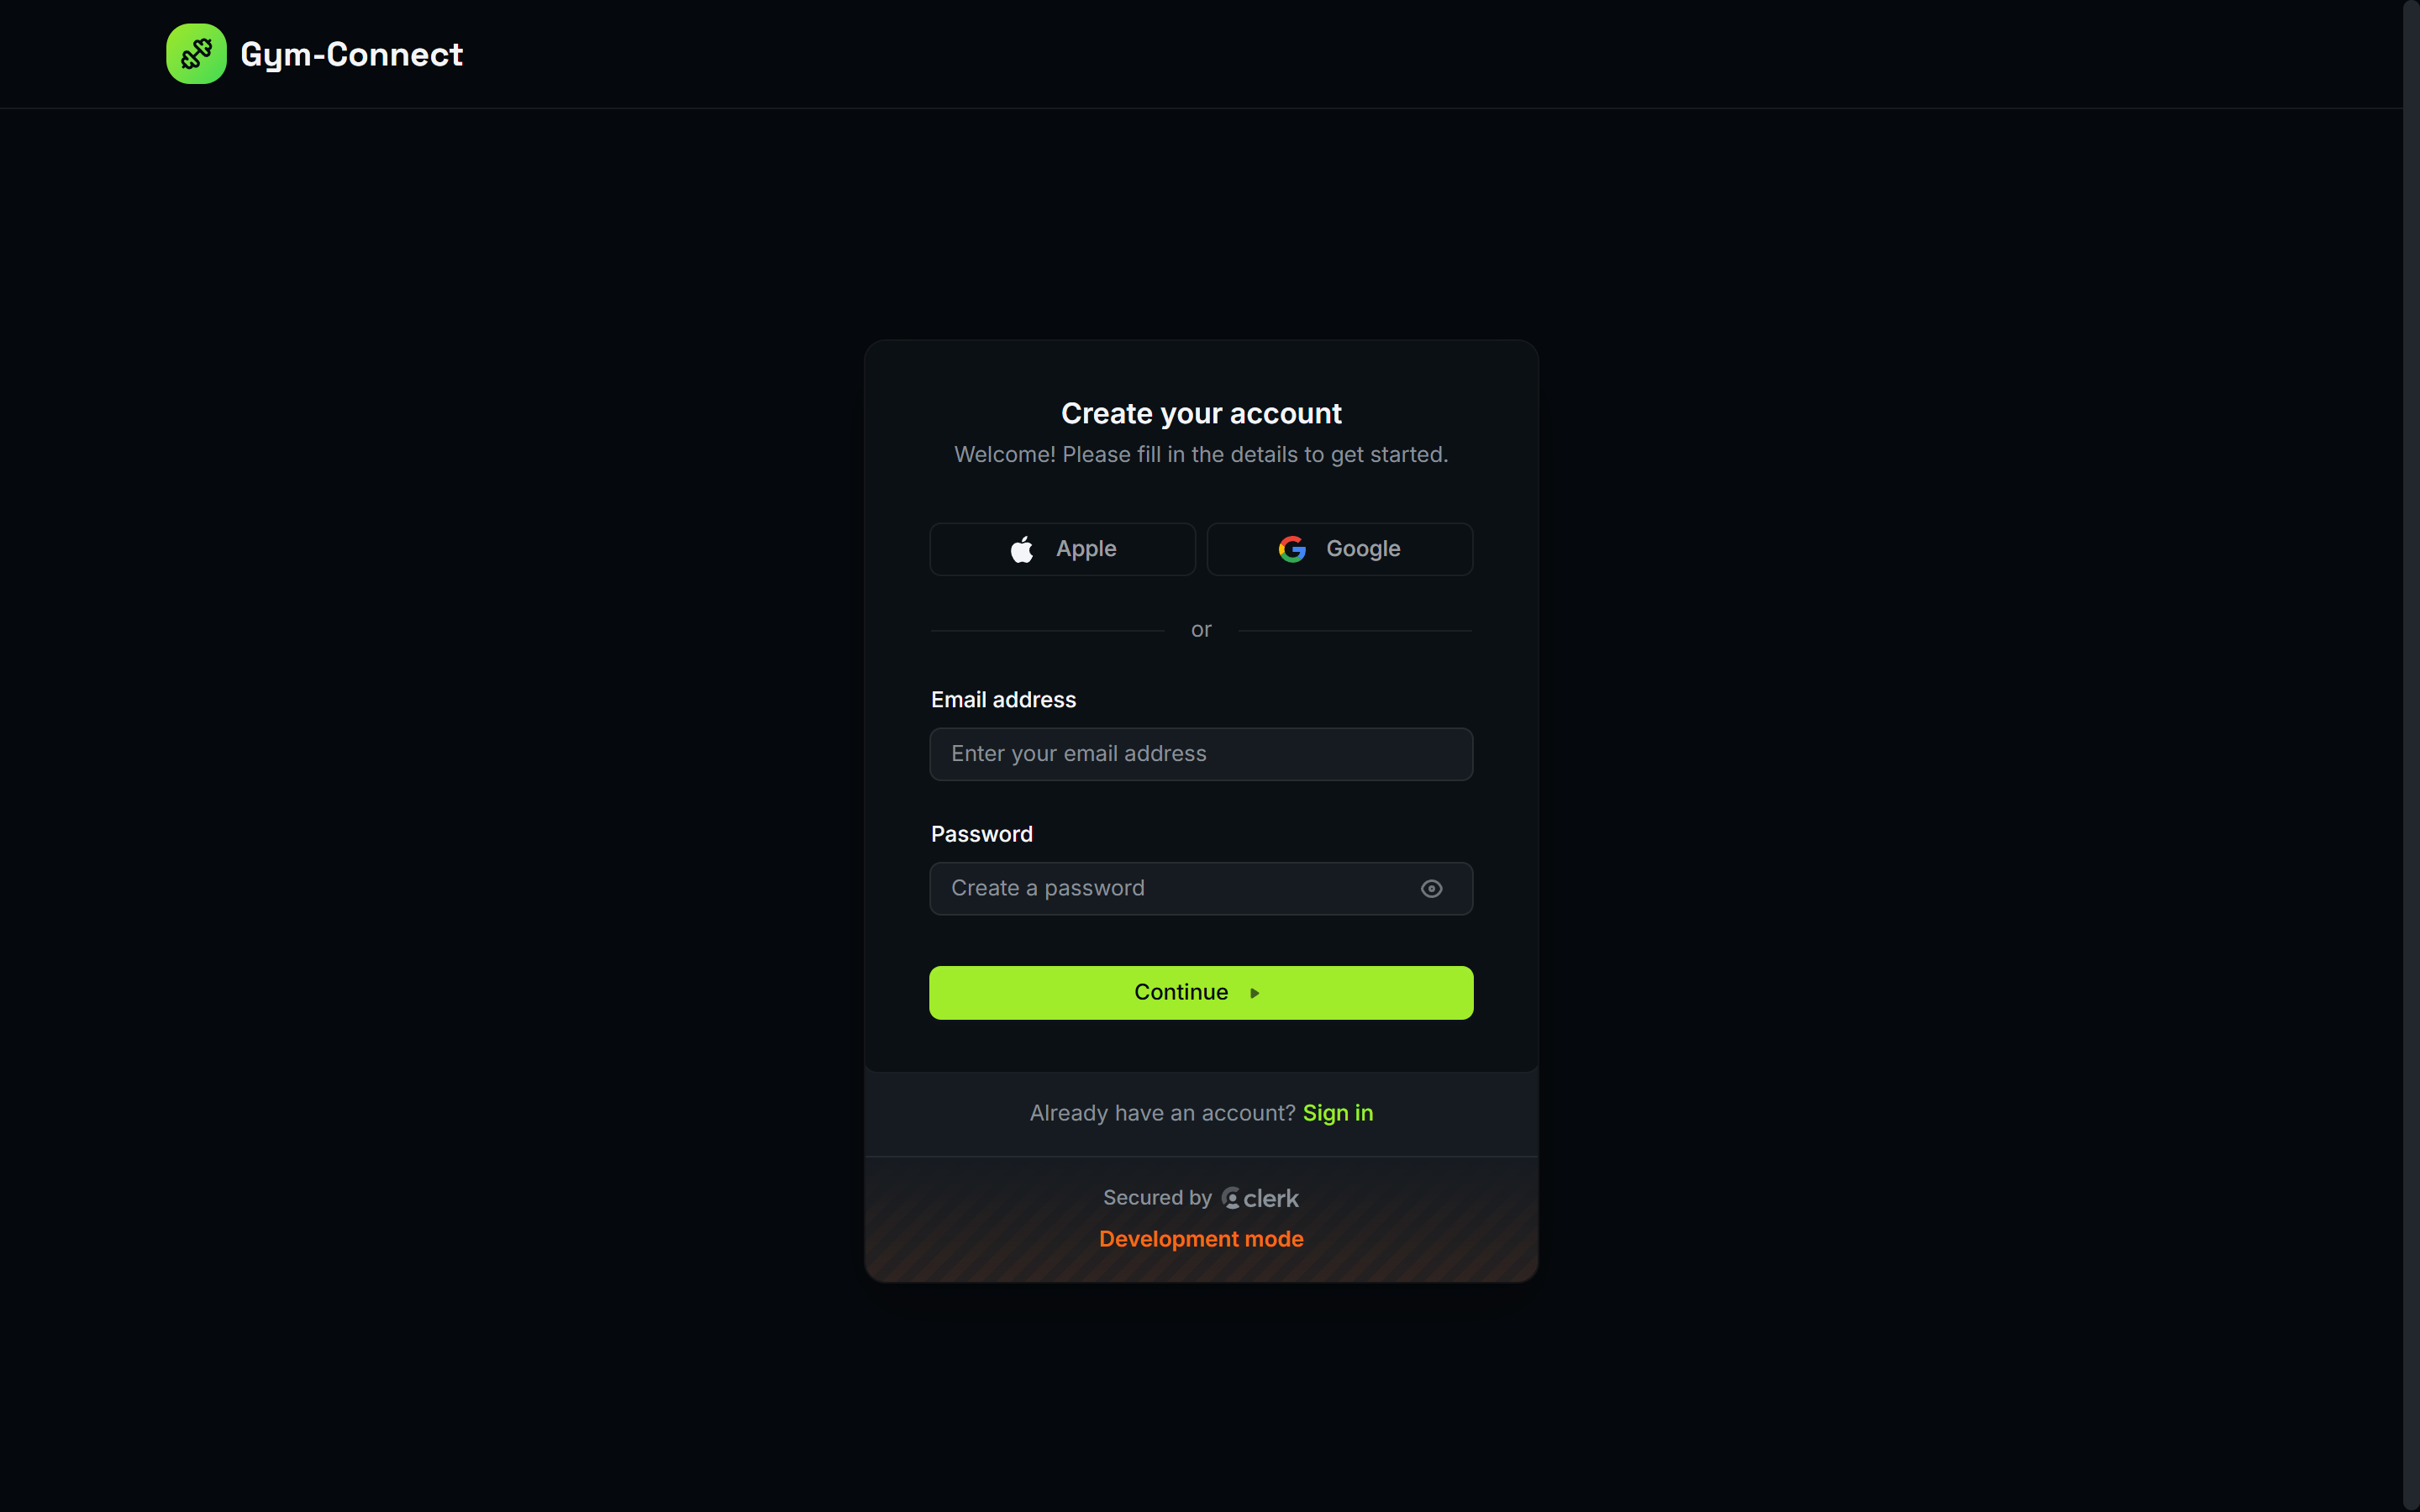
\includegraphics[width=\textwidth]{register.png}
  \caption{Pagina de \^ inregistrare}
  \label{fig:register}
\end{figure}

\section{Gestionarea rutinelor (Splits)}

Dup\u a autentificare, utilizatorul ajunge la pagina de rutine
(figura~\ref{fig:splits}). Aici sunt afi\c sate toate \c sabloanele de
antrenament salvate, fiecare cu exerci\c tiile sale. De pe acest ecran se
poate crea o rutin\u a nou\u a, edita sau \c sterge una existent\u a, ori porni
direct un antrenament.

\begin{figure}[H]
  \centering
  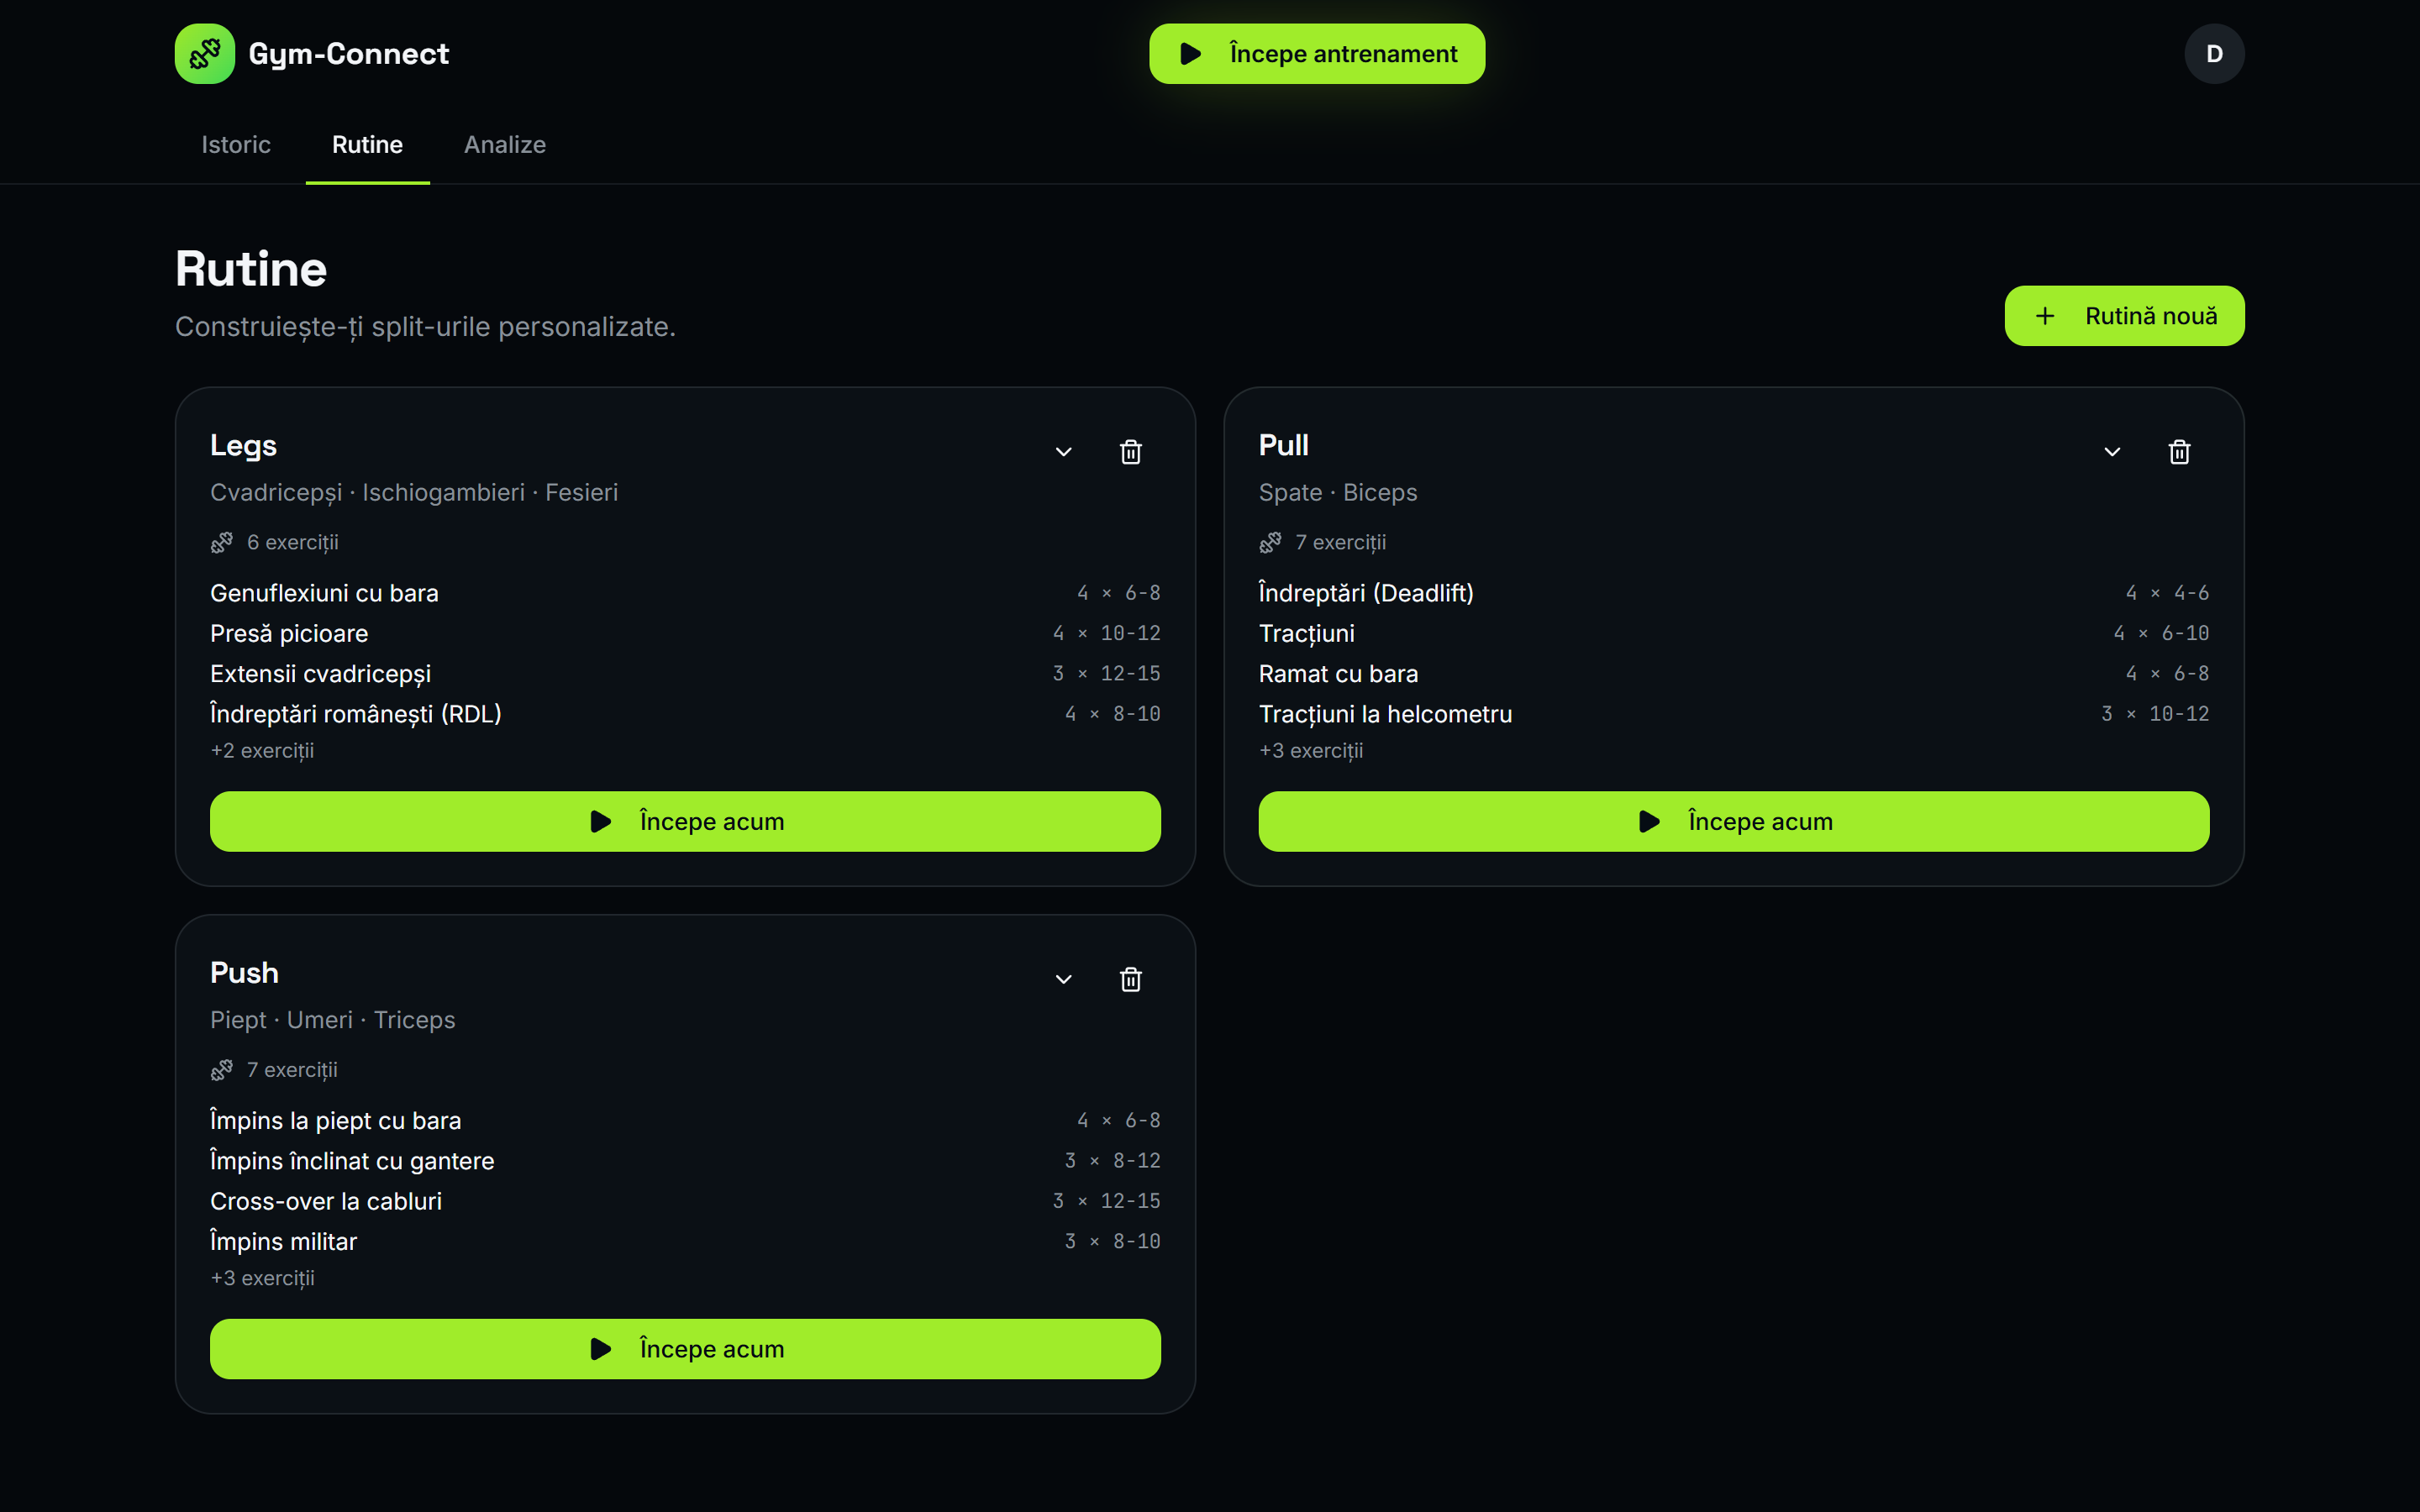
\includegraphics[width=\textwidth]{splits.png}
  \caption{Pagina de gestionare a rutinelor}
  \label{fig:splits}
\end{figure}

\subsection{Crearea unei rutine}

Crearea unei rutine se face \^ intr-un formular dedicat
(figura~\ref{fig:split-create}), \^ in care utilizatorul d\u a un nume rutinei,
o descriere op\c tional\u a \c si adaug\u a exerci\c tii. Pentru fiecare exerci\c tiu
se stabilesc num\u arul de seturi \c tint\u a \c si intervalul de repeti\c tii dorit.

\begin{figure}[H]
  \centering
  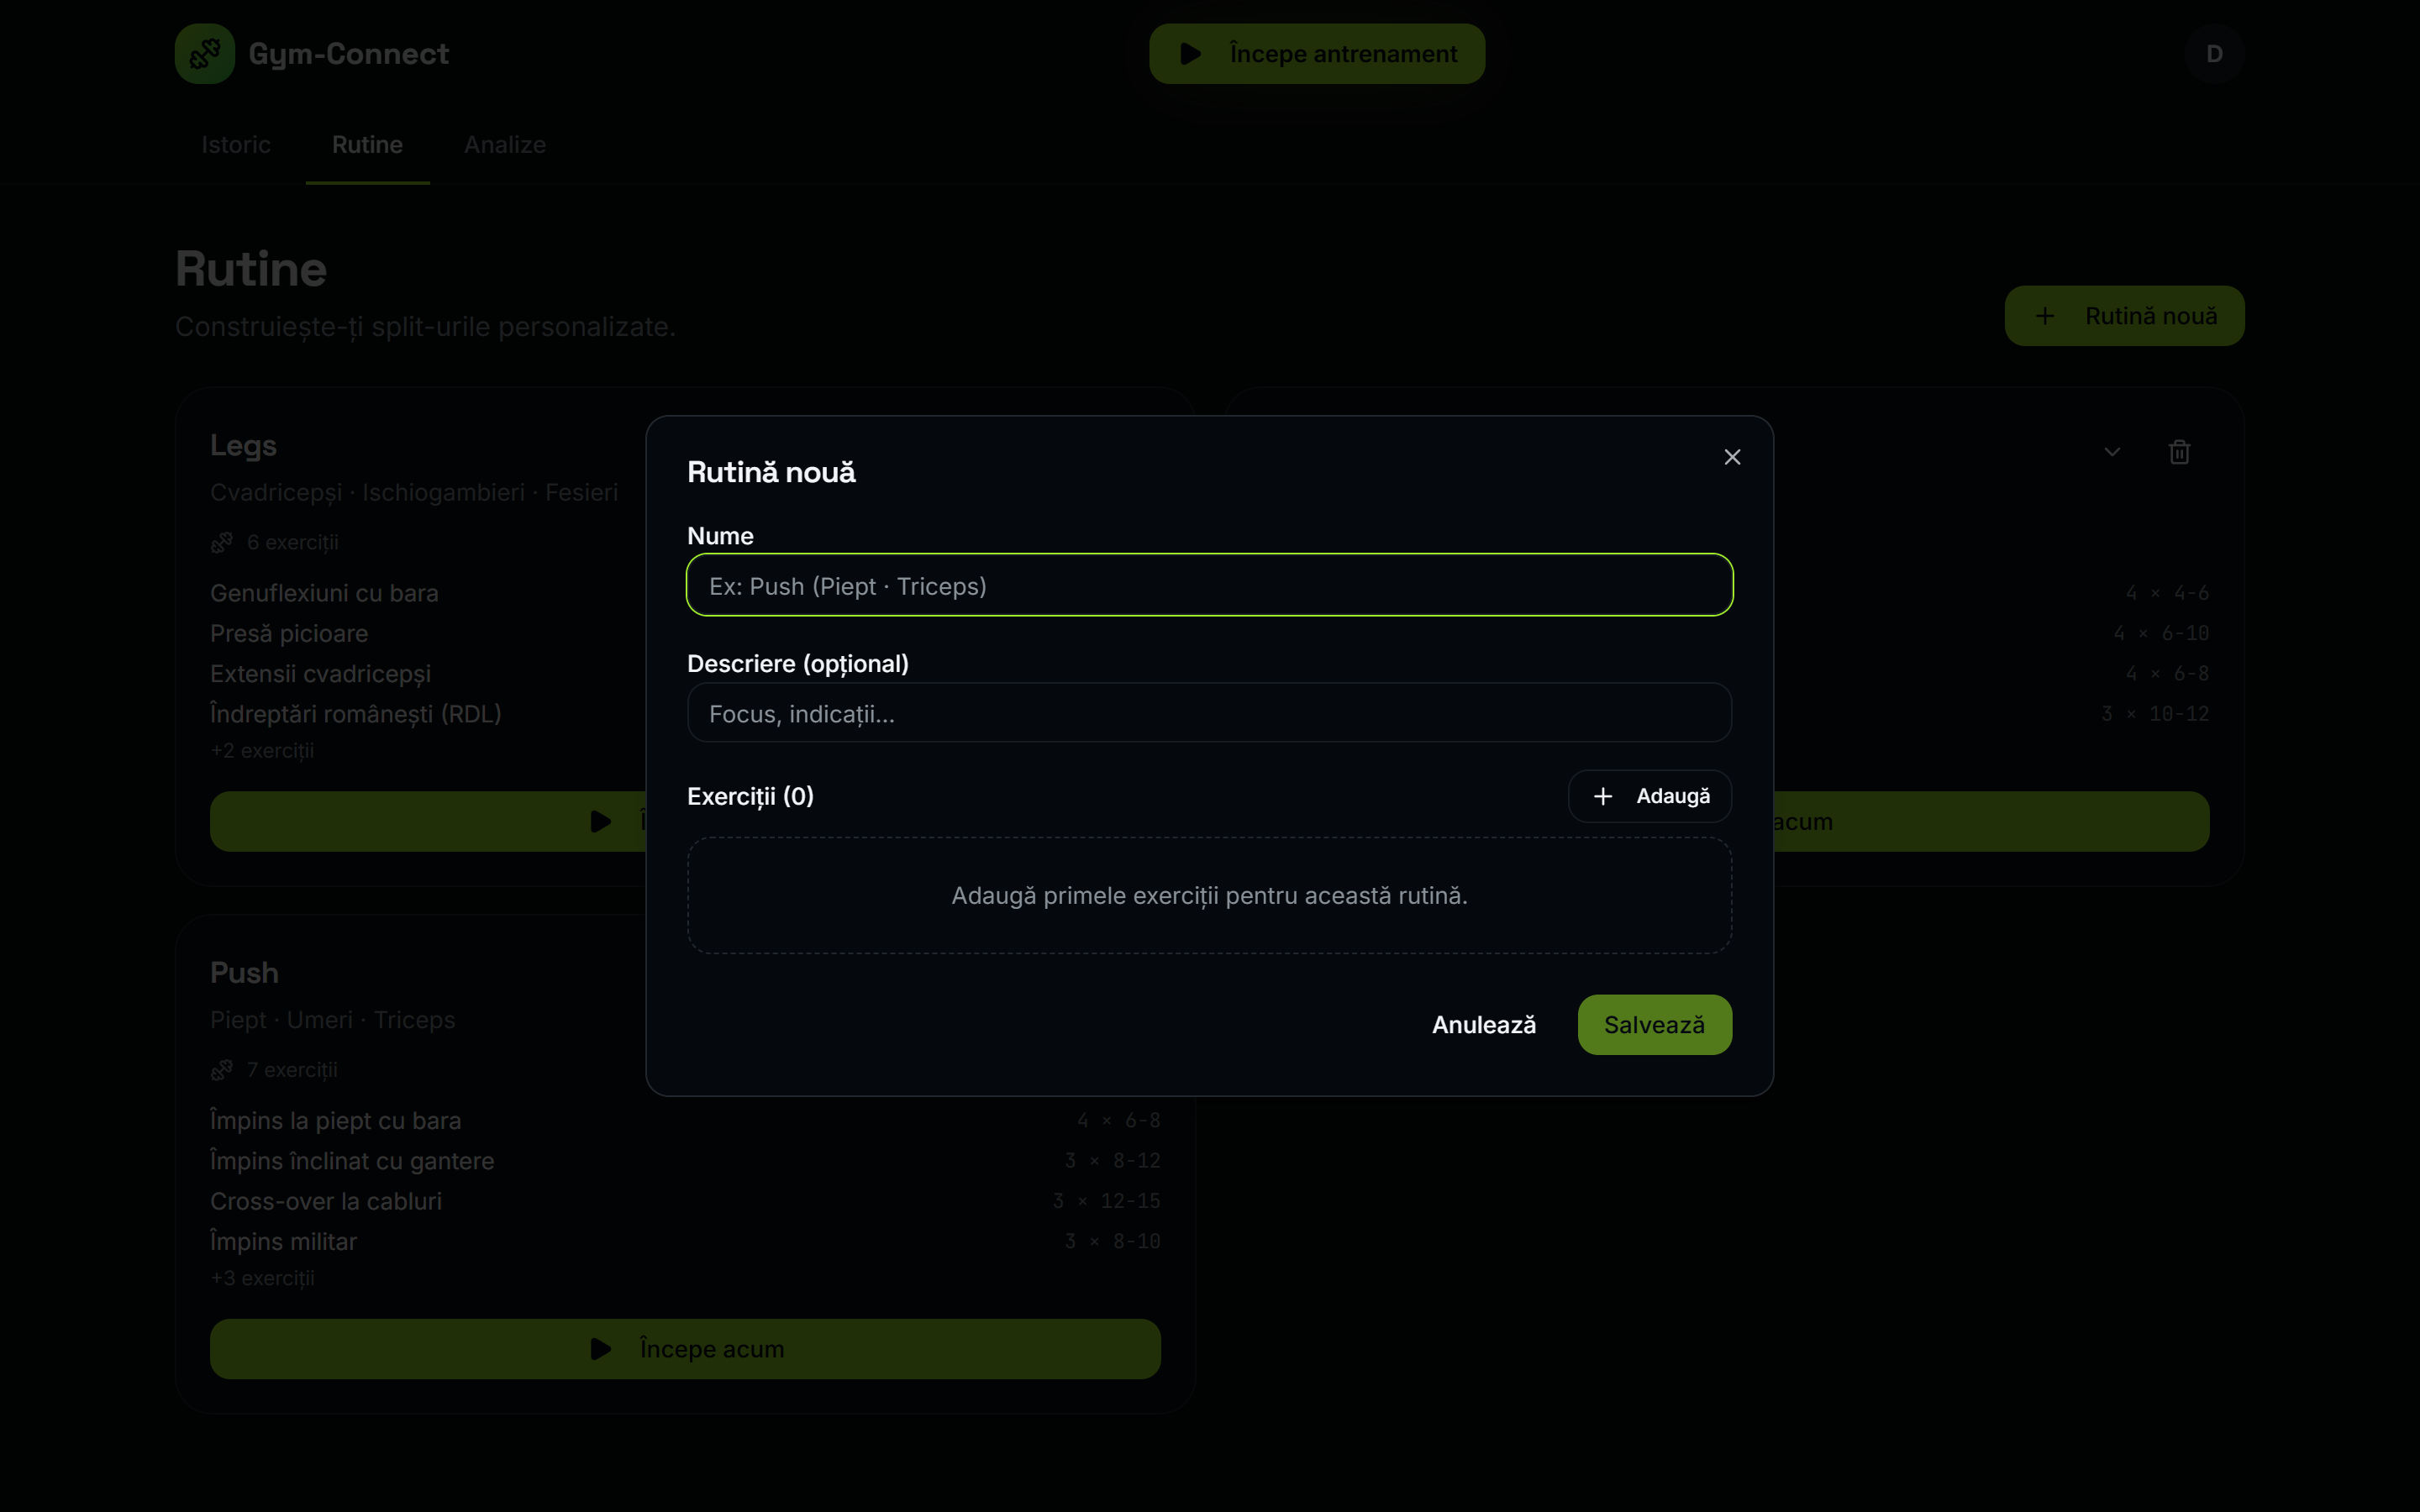
\includegraphics[width=\textwidth]{split-create.png}
  \caption{Crearea unei rutine}
  \label{fig:split-create}
\end{figure}

\subsection{Selectorul de exerci\c tii}

Ad\u augarea exerci\c tiilor se face printr-un selector
(figura~\ref{fig:exercise-picker}) care afi\c seaz\u a biblioteca de exerci\c tii
grupat\u a pe grupe musculare. Utilizatorul poate c\u auta rapid un exerci\c tiu
dup\u a nume \c si \^ il adaug\u a \^ in rutin\u a cu un singur click.

\begin{figure}[H]
  \centering
  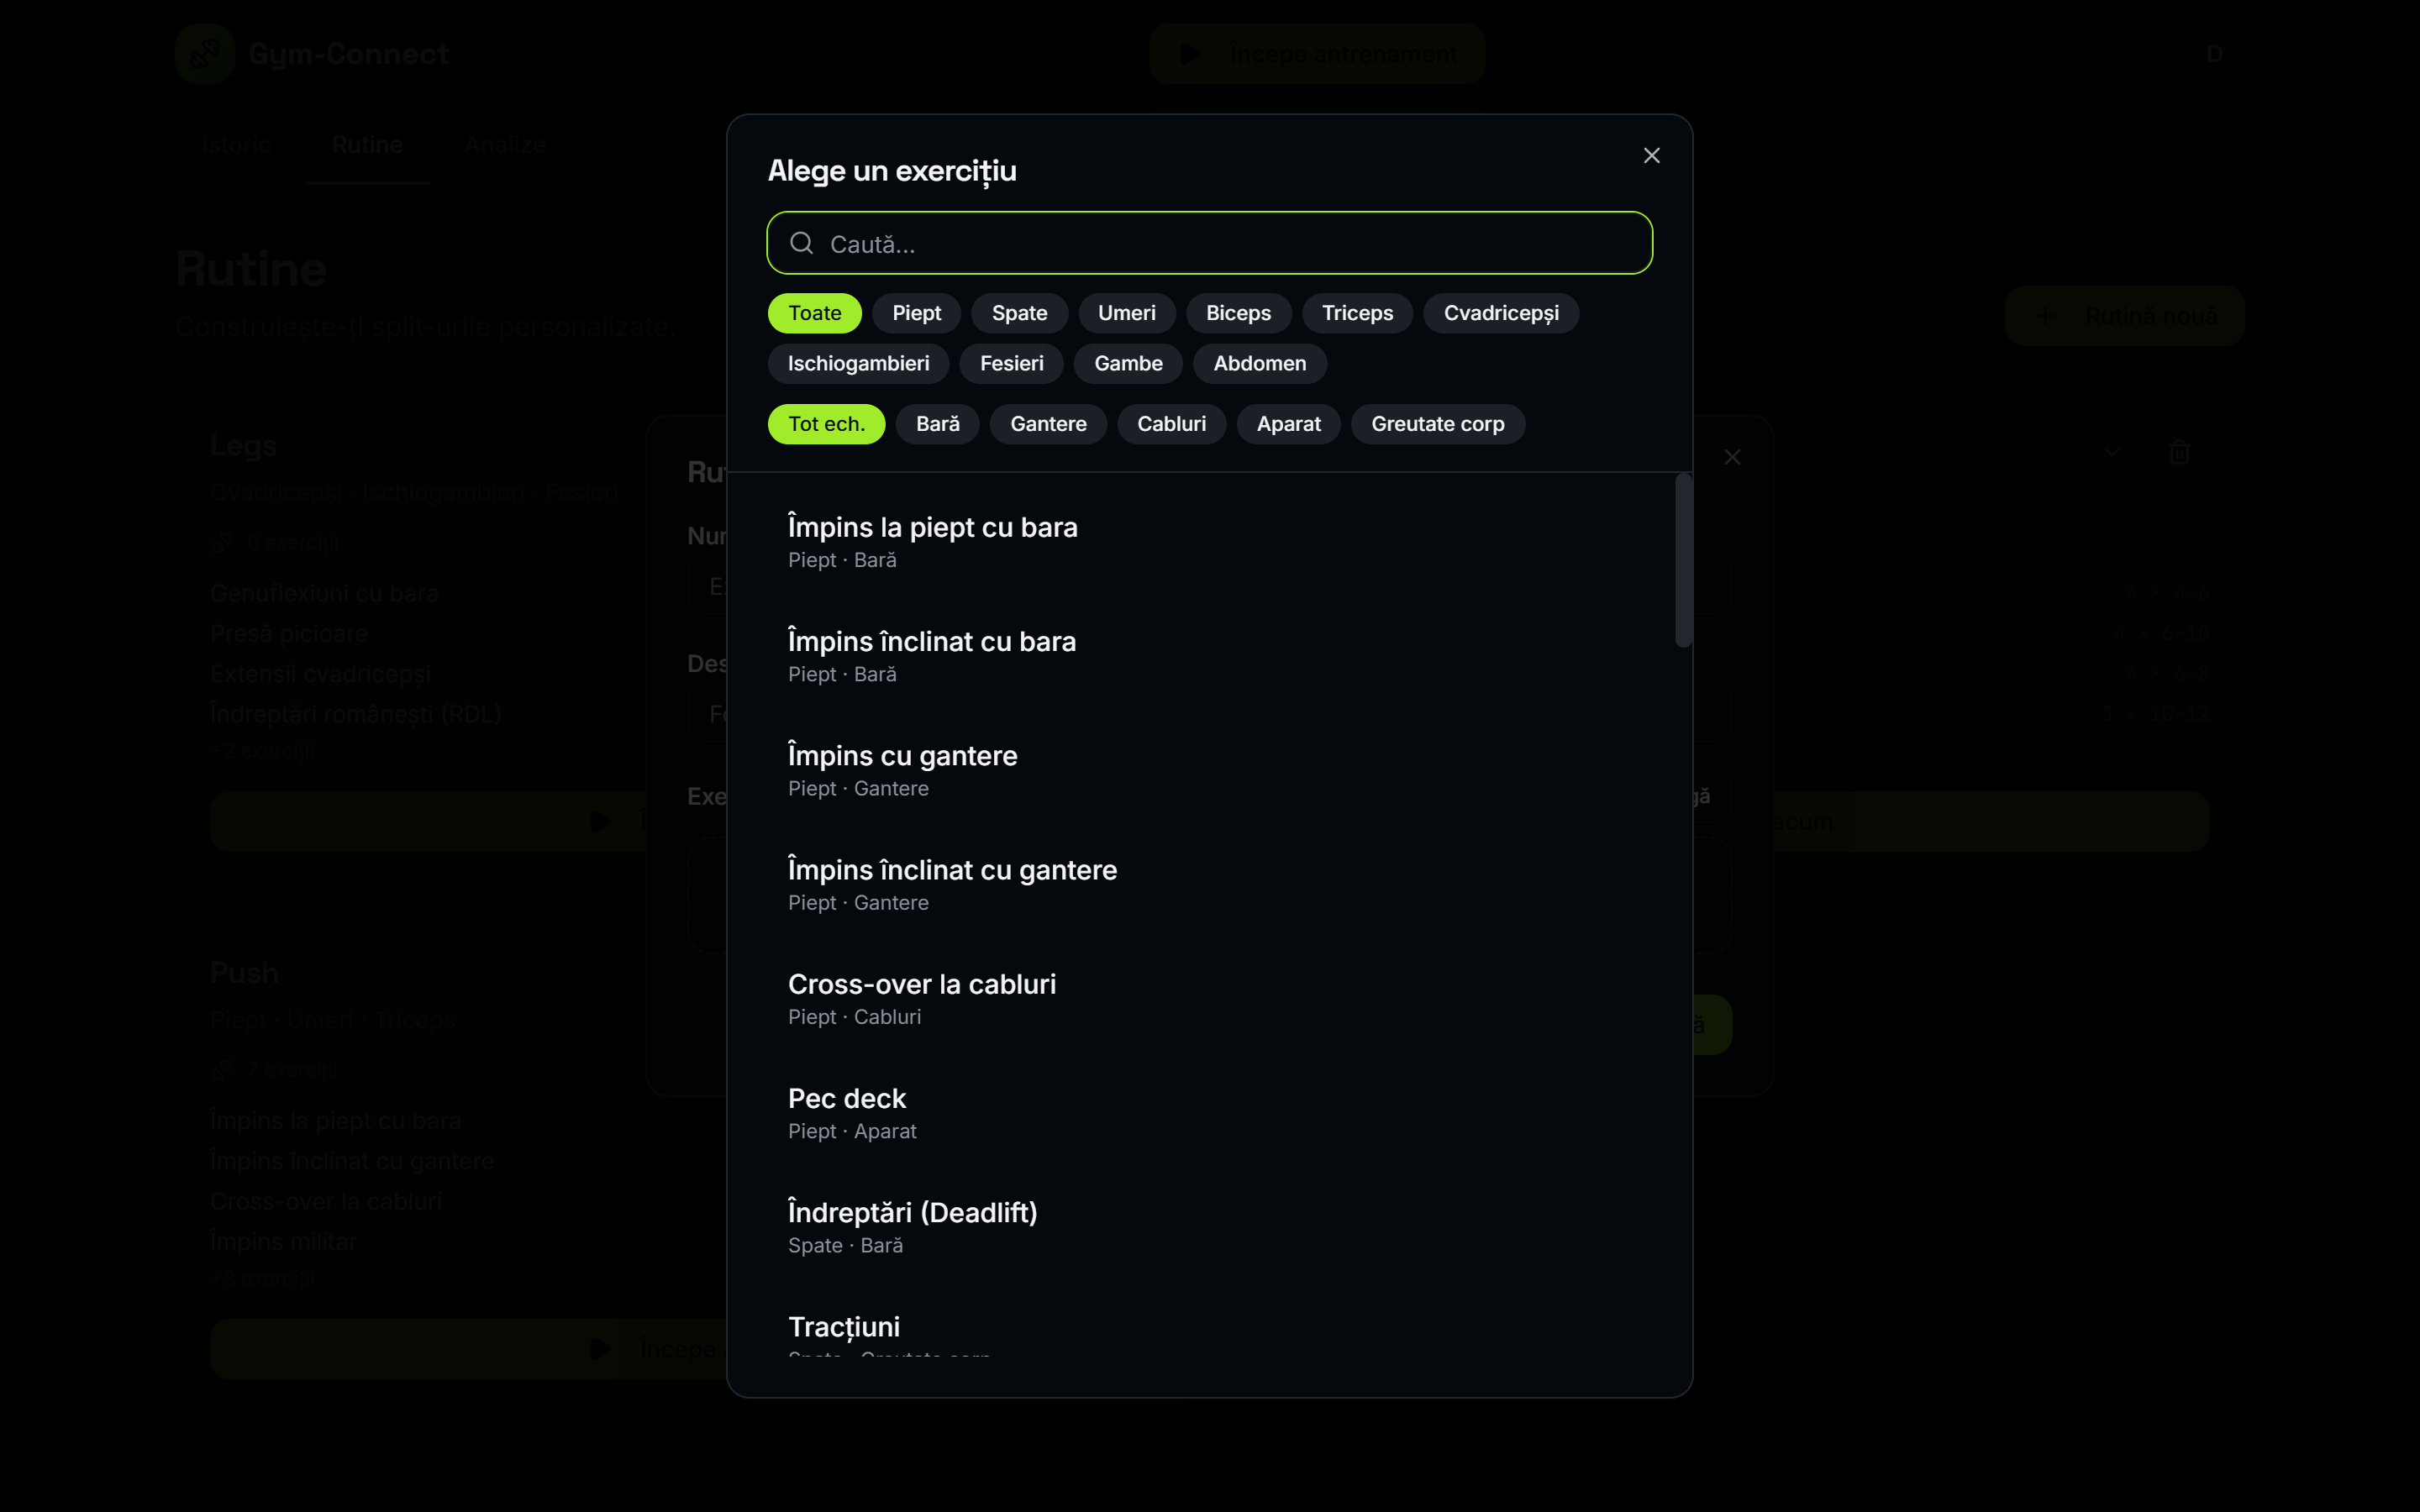
\includegraphics[width=\textwidth]{exercise-picker.png}
  \caption{Selectorul de exerci\c tii}
  \label{fig:exercise-picker}
\end{figure}

\section{Sesiunea de antrenament (Workout)}

Modulul de antrenament (figura~\ref{fig:workout}) este inima aplica\c tiei --
ecranul pe care utilizatorul \^ il folose\c ste efectiv \^ in sal\u a. Aici se
desf\u a\c soar\u a sesiunea \^ in timp real: exerci\c tiile din rutin\u a sunt
afi\c sate pe r\^ and, iar seturile se completeaz\u a pe m\u asur\u a ce sunt
efectuate.

\begin{figure}[H]
  \centering
  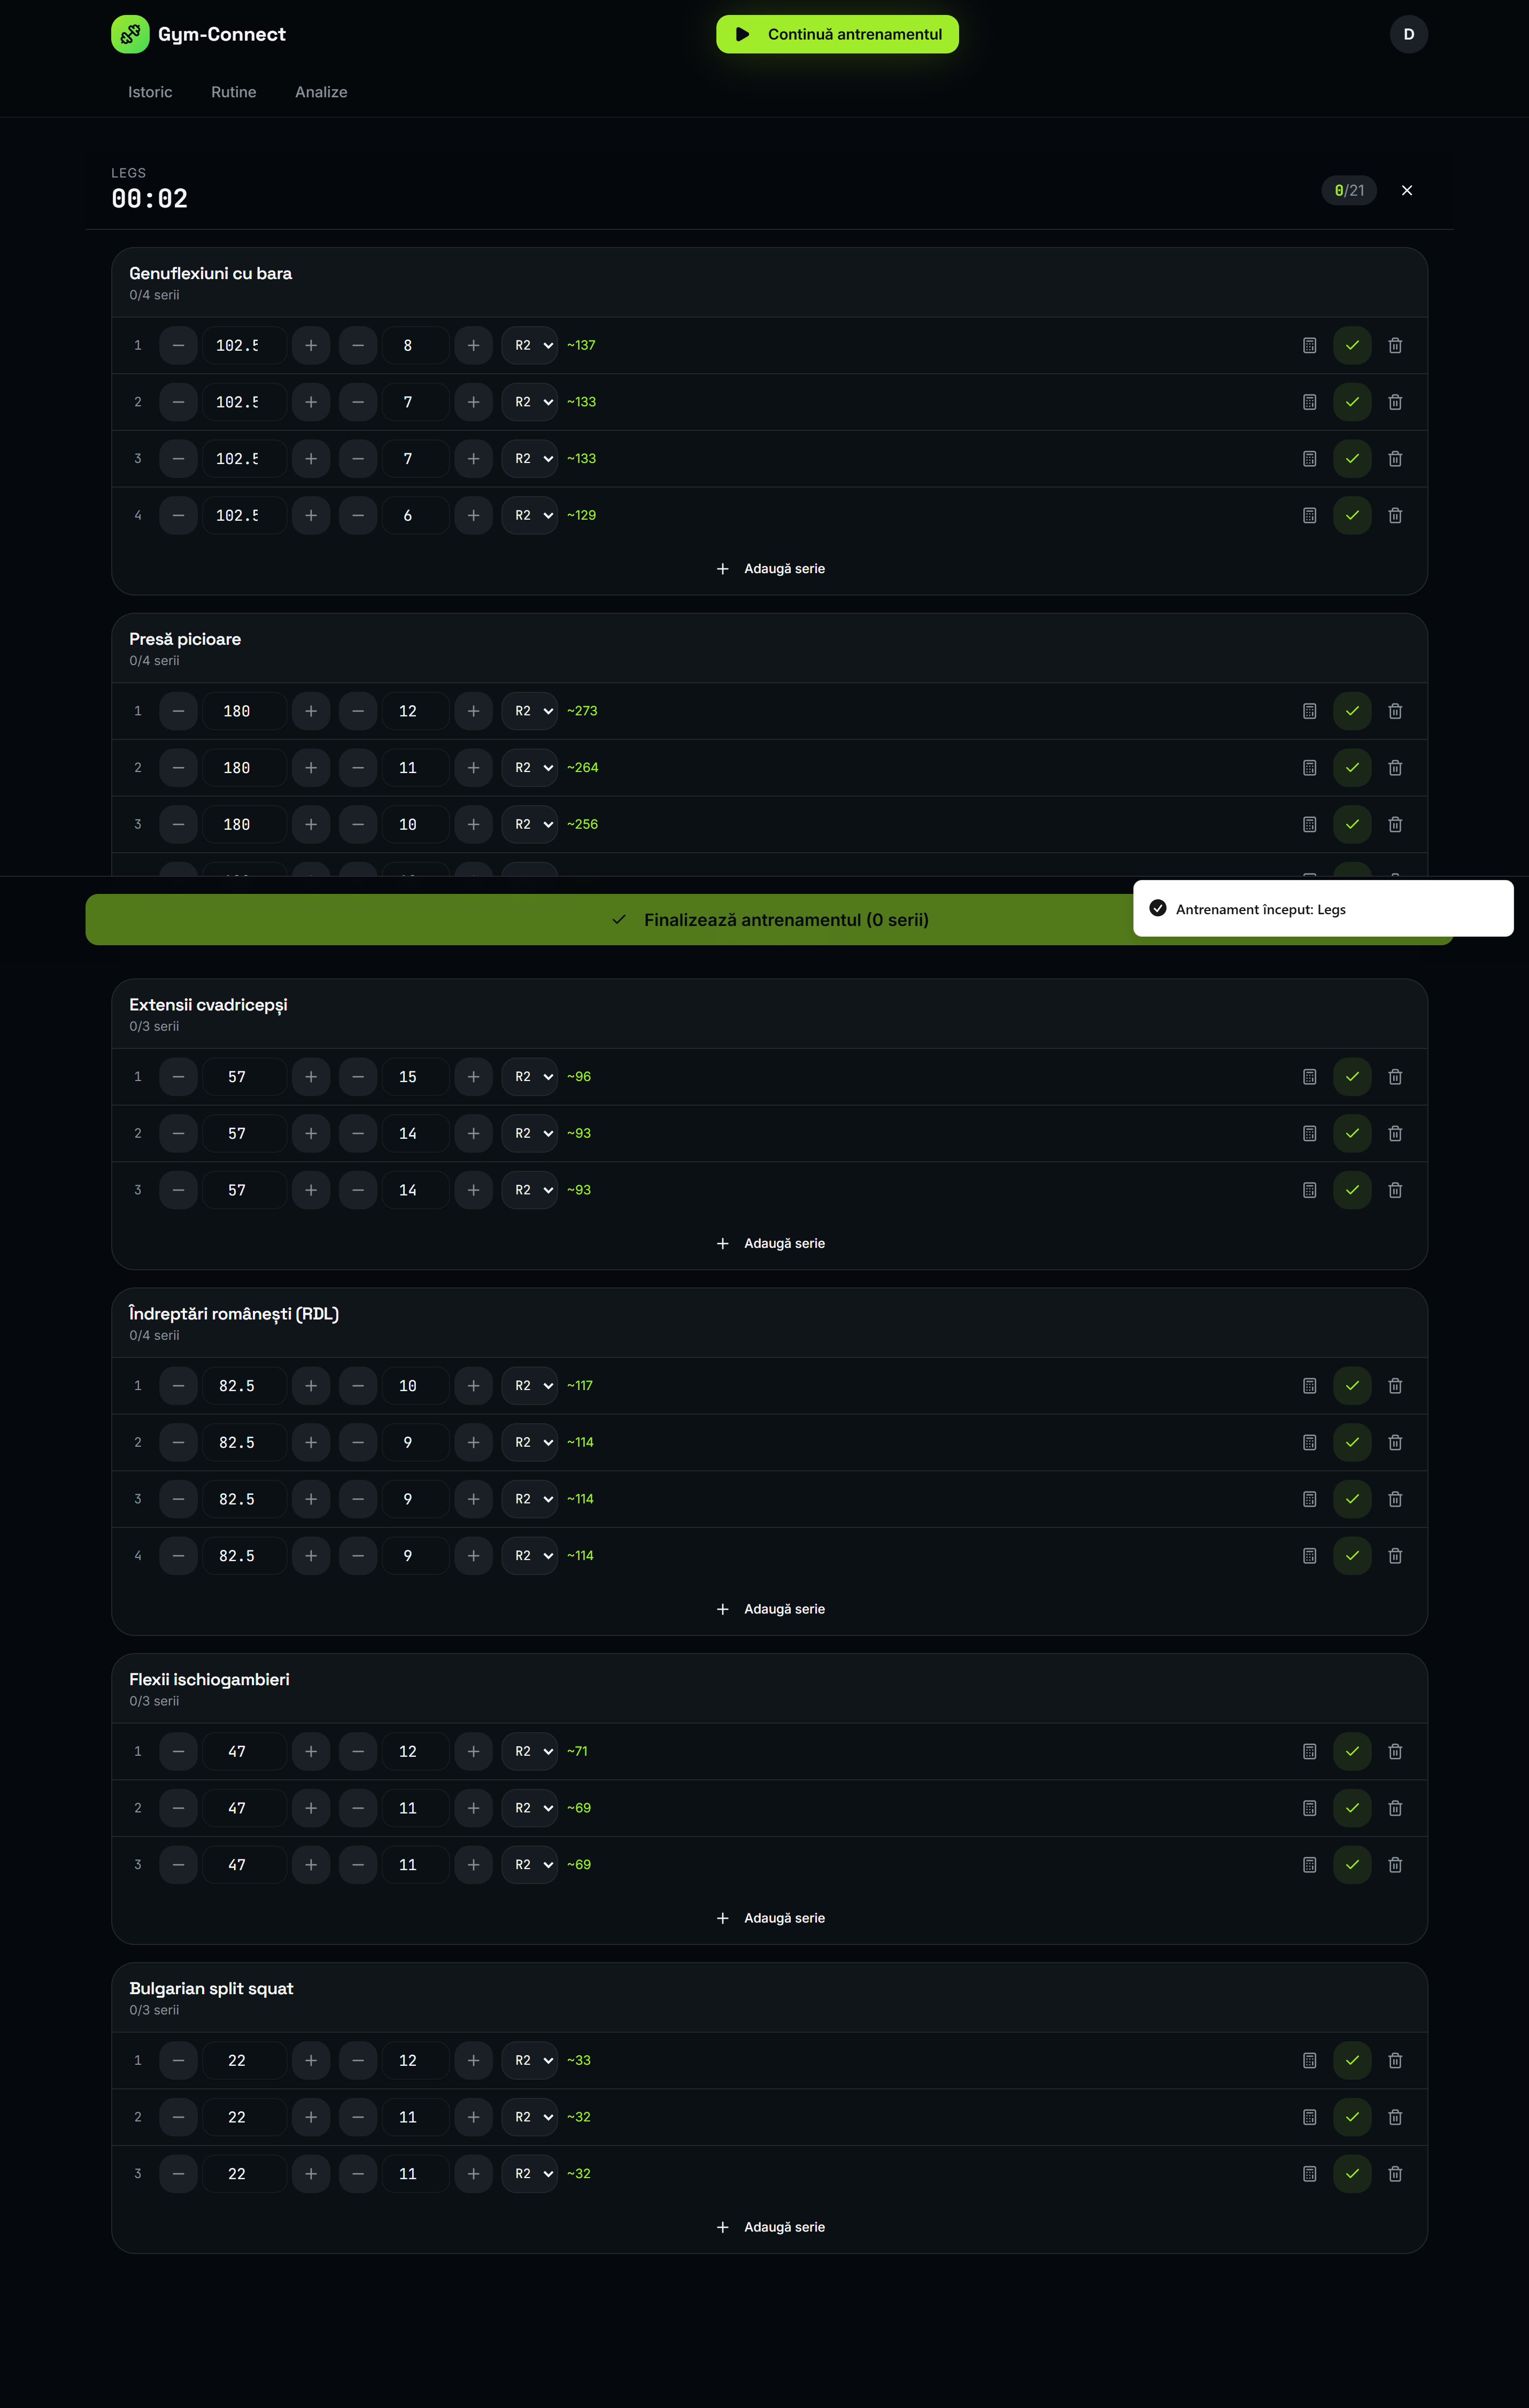
\includegraphics[height=0.78\textheight]{workout.png}
  \caption{Sesiunea de antrenament}
  \label{fig:workout}
\end{figure}

\subsection{Cronometrul \c si indicatorul de progres}

Dup\u a fiecare set, aplica\c tia porne\c ste automat un cronometru de odihn\u a
(figura~\ref{fig:timer}), \^ inso\c tit de un indicator care arat\u a c\^ ate
seturi au fost finalizate din totalul planificat. Acest detaliu m\u arunt
conteaz\u a \^ in practic\u a: nu mai trebuie s\u a urm\u are\c sti pauza separat,
pe telefon.

\begin{figure}[H]
  \centering
  
\includegraphics[width=\textwidth]{timer.png}
  \caption{Cronometrul \c si indicatorul de progres}
  \label{fig:timer}
\end{figure}

\subsection{Gestionarea seturilor}

\^ Inregistrarea propriu-zis\u a a seturilor este prezentat\u a \^ in
figura~\ref{fig:sets}. Pentru fiecare exerci\c tiu, utilizatorul introduce
greutatea \c si num\u arul de repeti\c tii, fiecare set ap\u ar\^ and pe un r\^ and
separat, u\c sor de urm\u arit.

\begin{figure}[H]
  \centering
  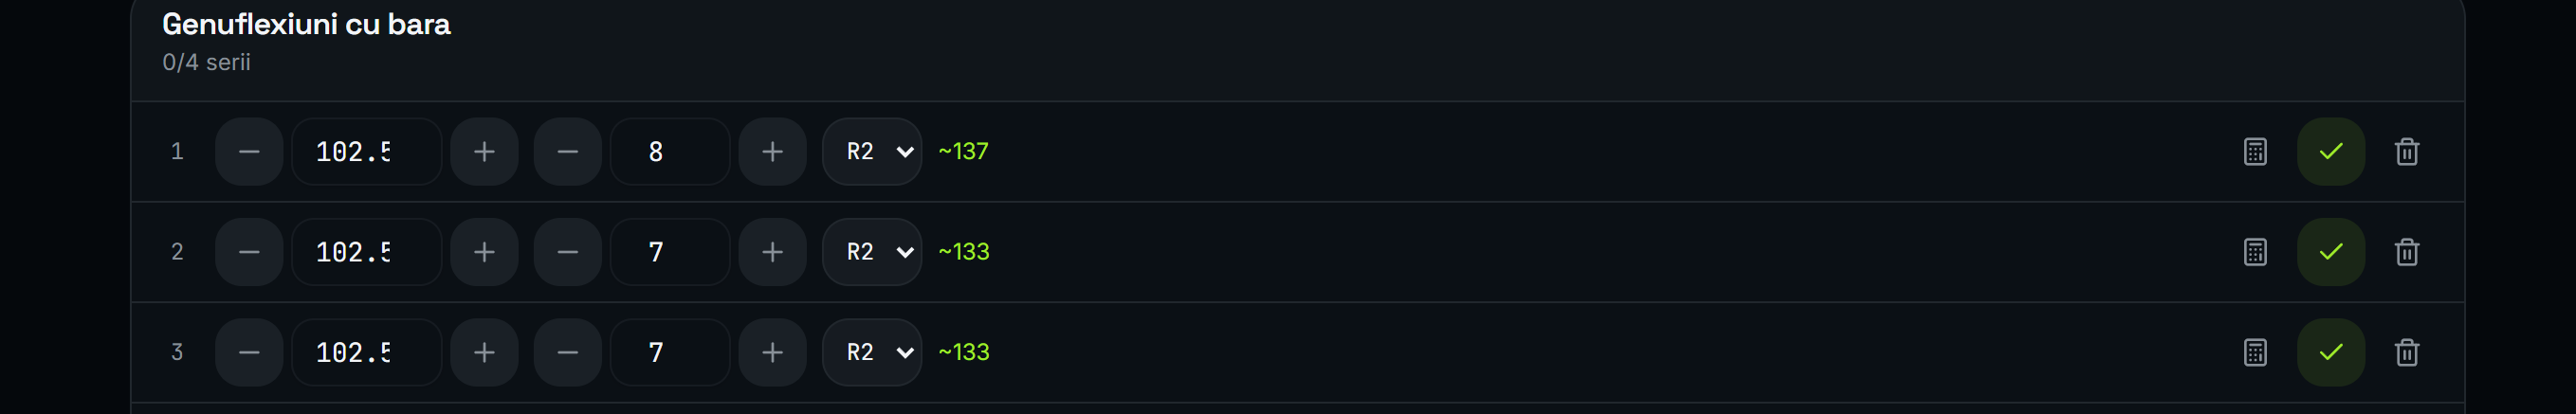
\includegraphics[width=\textwidth]{sets.png}
  \caption{Gestionarea seturilor}
  \label{fig:sets}
\end{figure}

\subsection{Calculatorul de pl\u aci}

Un instrument pe care \^ il consider deosebit de util este calculatorul de
pl\u aci (figura~\ref{fig:plates}). Pornind de la greutatea \c tint\u a, acesta
calculeaz\u a exact ce discuri trebuie puse pe fiecare cap\u at al barei de
20~kg, sc\u ap\^ andu-l pe utilizator de un calcul mental incomod \^ in mijlocul
antrenamentului.

\begin{figure}[H]
  \centering
  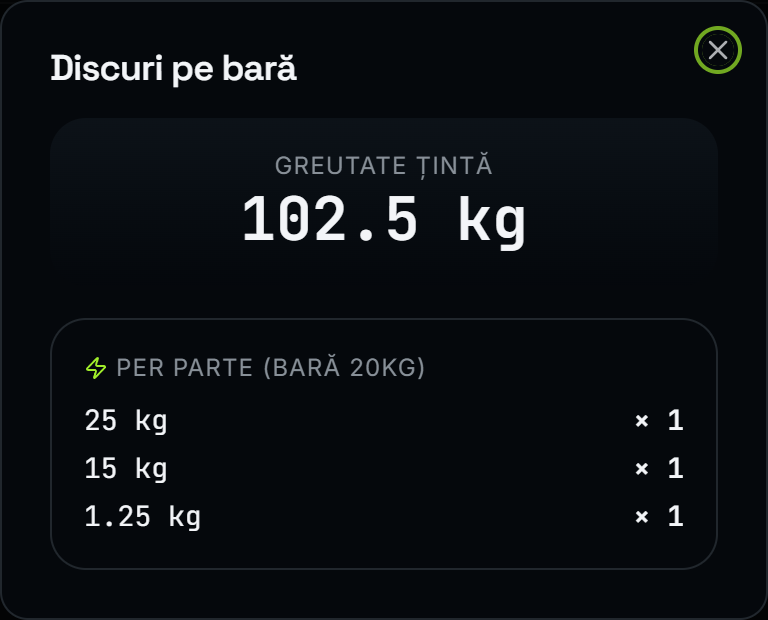
\includegraphics[width=0.5\textwidth]{plates.png}
  \caption{Calculatorul de pl\u aci}
  \label{fig:plates}
\end{figure}

\subsection{Indicatori de intensitate: RIR \c si 1RM}

Figura~\ref{fig:intensity} arat\u a cum aplica\c tia capteaz\u a intensitatea
efortului. Pe l\^ ang\u a greutate \c si repeti\c tii, fiecare set are asociat\u a
o valoare RIR (\textit{Reps in Reserve}), iar aplica\c tia calculeaz\u a \c si
afi\c seaz\u a imediat 1RM-ul estimat pentru setul respectiv.

\begin{figure}[H]
  \centering
  
\includegraphics[width=\textwidth]{intensity.png}
  \caption{Indicatori de intensitate: RIR \c si 1RM}
  \label{fig:intensity}
\end{figure}

\section{Istoricul antrenamentelor (History)}

Istoricul antrenamentelor (figura~\ref{fig:history}) func\c tioneaz\u a ca un
jurnal: toate sesiunile anterioare sunt listate cronologic, \^ impreun\u a cu
statistici de ansamblu precum volumul total ridicat \c si durata medie a unui
antrenament. De aici utilizatorul \^ i\c si poate urm\u ari activitatea pe termen
lung.

\begin{figure}[H]
  \centering
  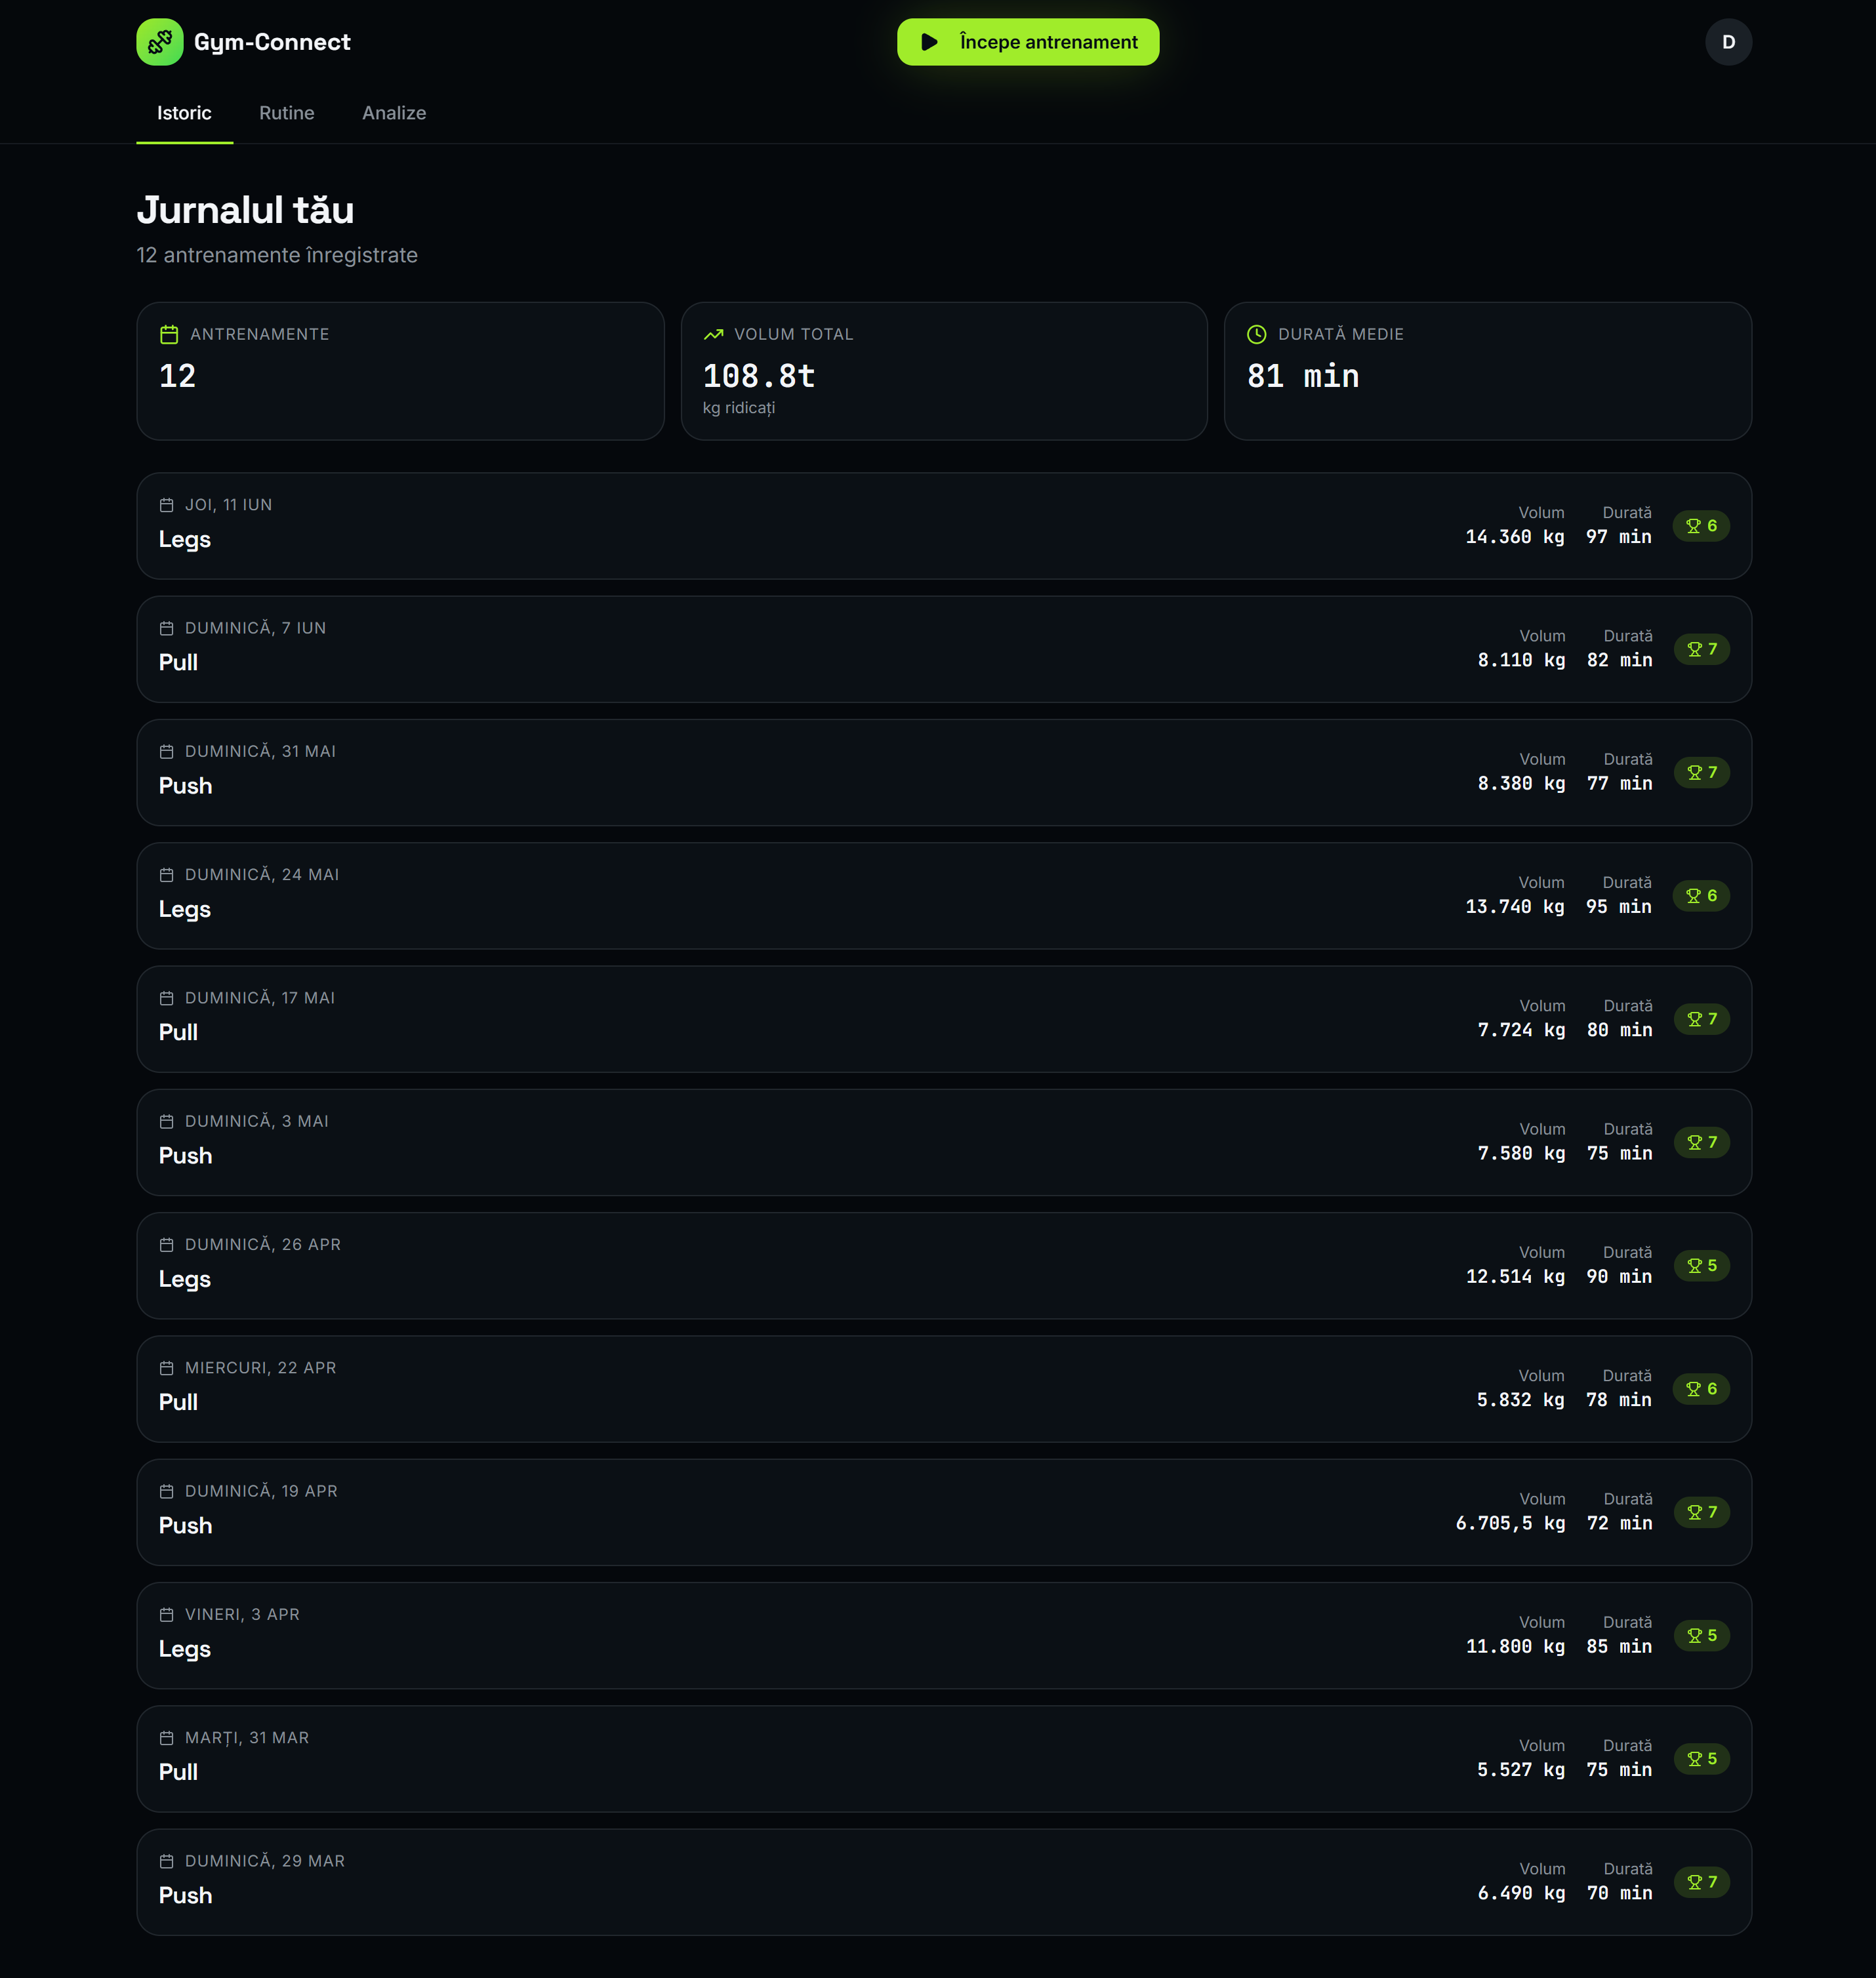
\includegraphics[width=0.8\textwidth]{history.png}
  \caption{Istoricul antrenamentelor}
  \label{fig:history}
\end{figure}

\section{Modulul de analitic\u a (Analytics)}

Modulul de analitic\u a (figura~\ref{fig:analytics}) este, \^ in opinia mea,
partea cea mai valoroas\u a a aplica\c tiei. El transform\u a datele brute din
istoric \^ in informa\c tie util\u a, prin dou\u a grafice principale \c si un
sistem de avertizare, pe care le detaliez \^ in continuare.

\begin{figure}[H]
  \centering
  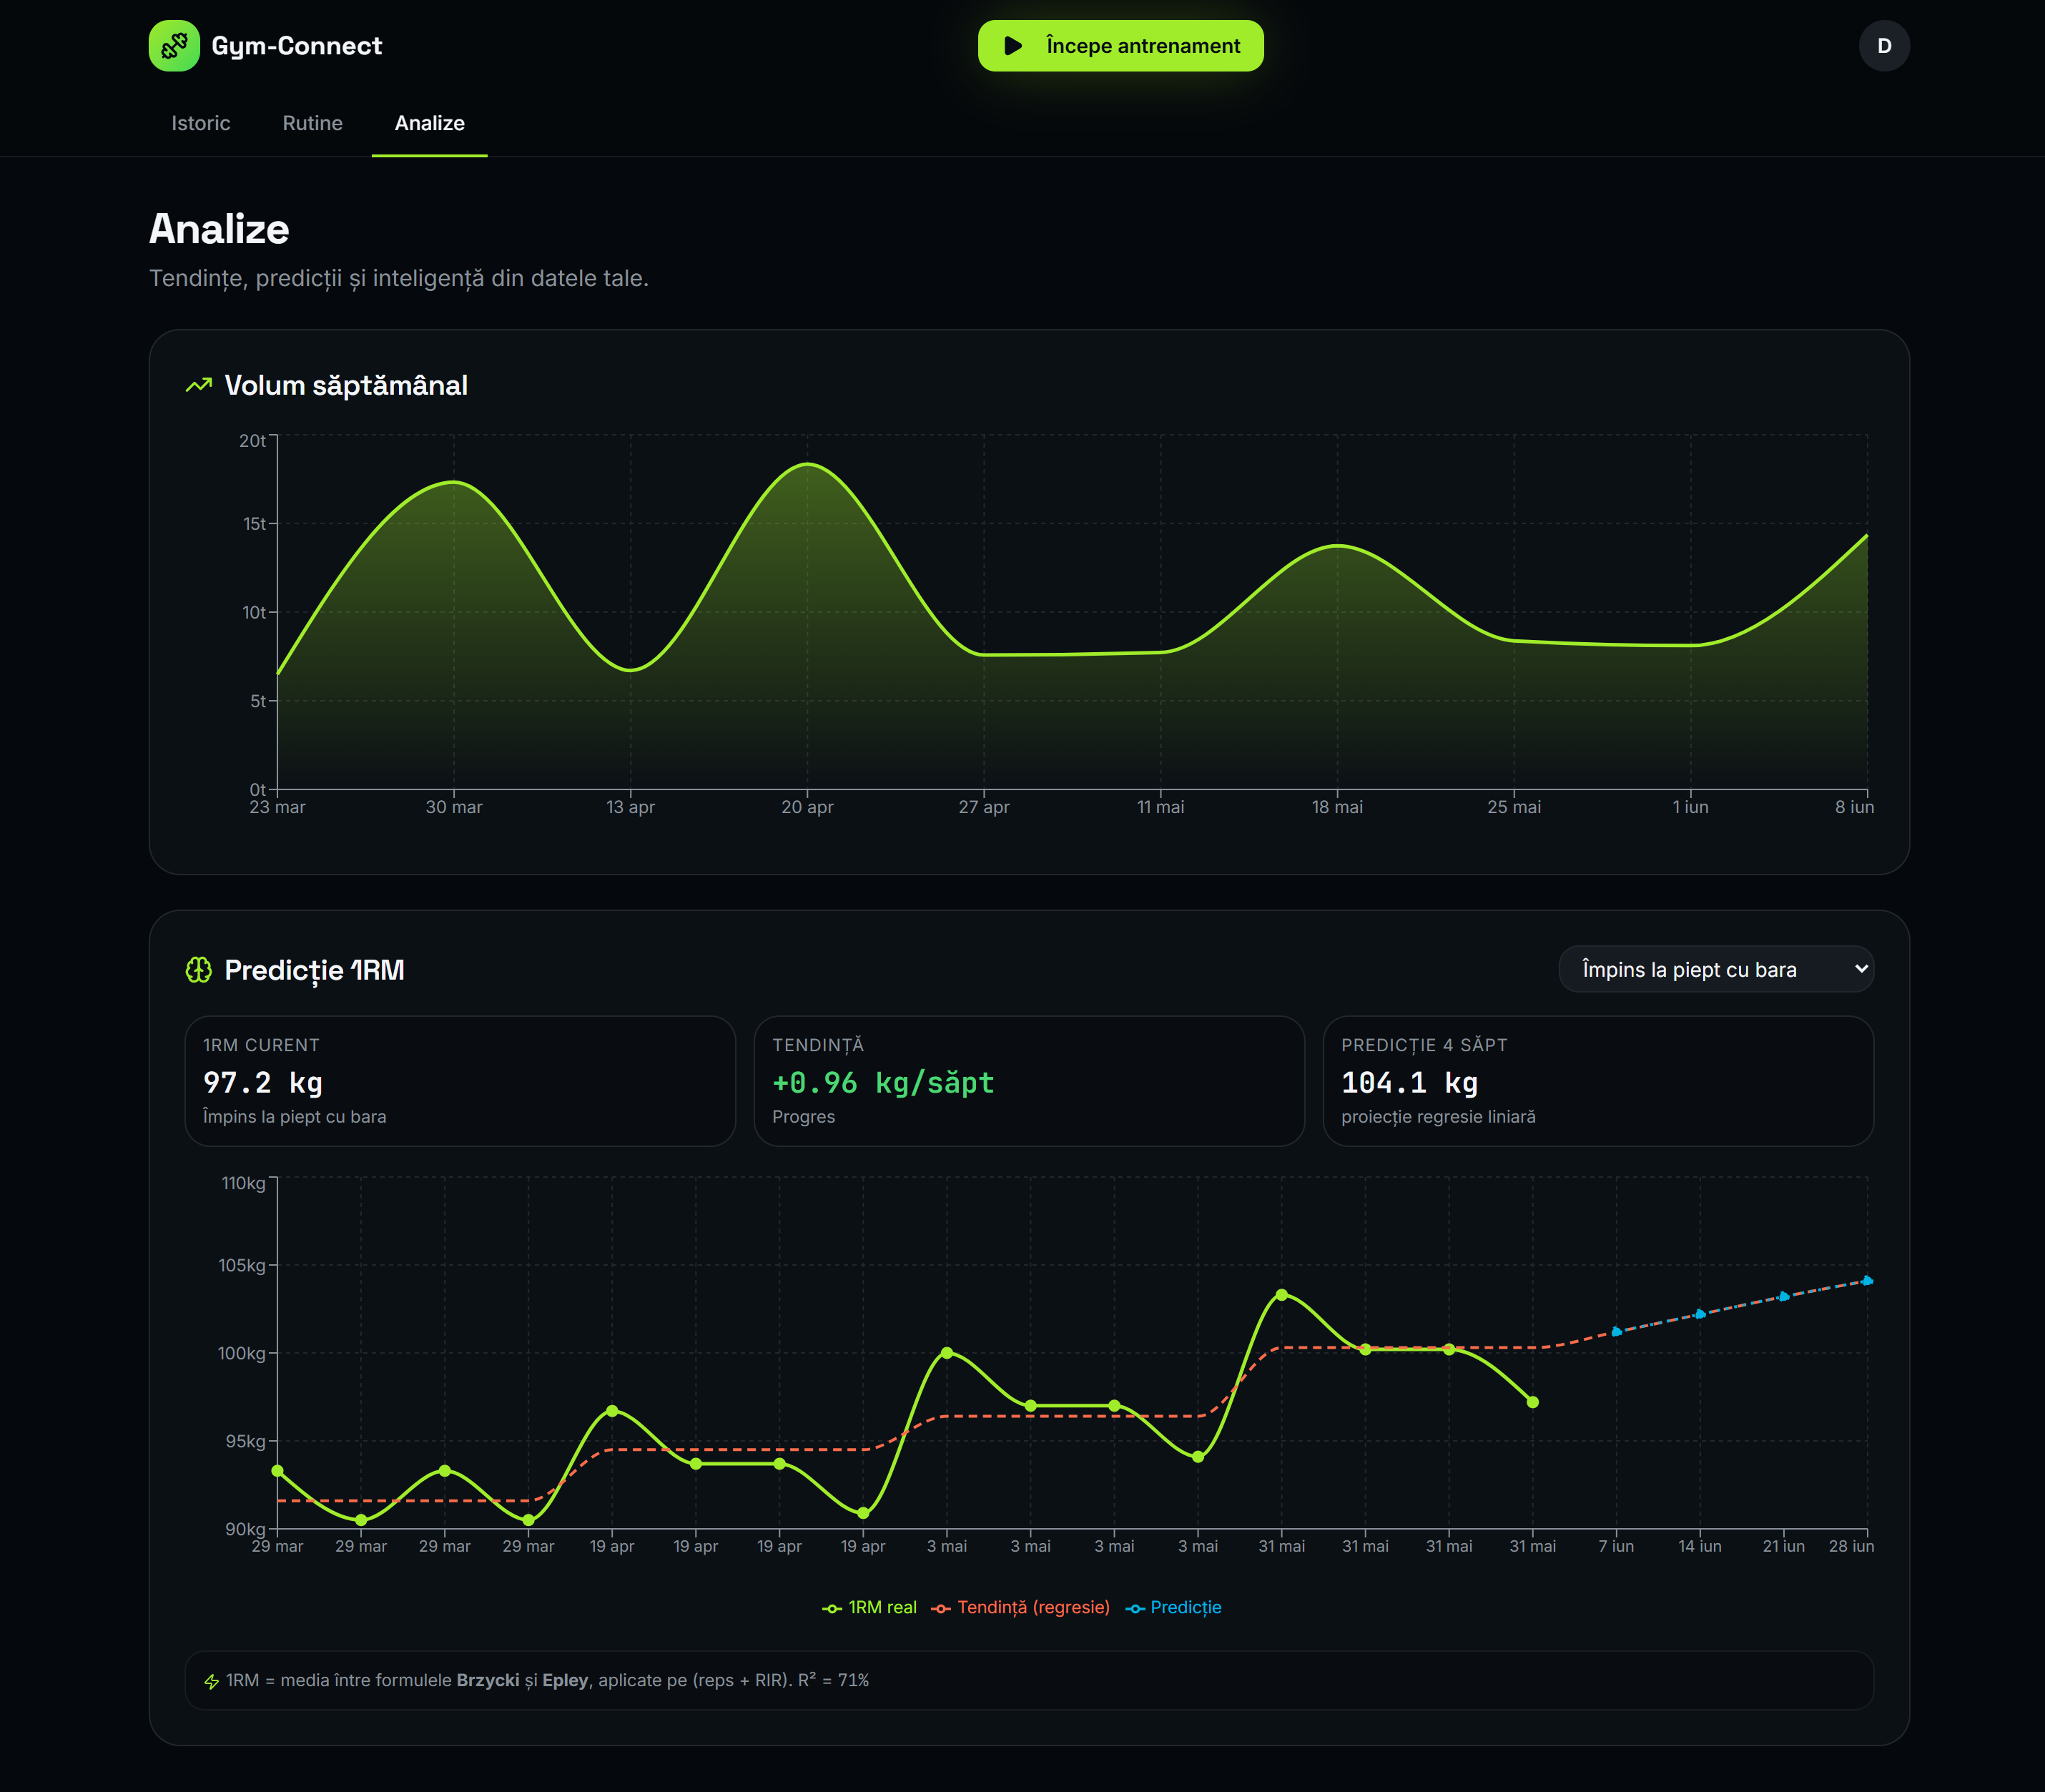
\includegraphics[width=\textwidth]{analytics.png}
  \caption{Modulul de analitic\u a}
  \label{fig:analytics}
\end{figure}

\subsection{Graficul volumului s\u apt\u am\^ anal}

Primul grafic (figura~\ref{fig:volume}) prezint\u a volumul total de
antrenament, agregat pe s\u apt\u am\^ ani. Vizualizarea ajut\u a utilizatorul
s\u a \^ in\c teleag\u a dac\u a \^ i\c si cre\c ste treptat \^ inc\u arc\u atura --
esen\c ta principiului \textit{progressive overload}.

\begin{figure}[H]
  \centering
  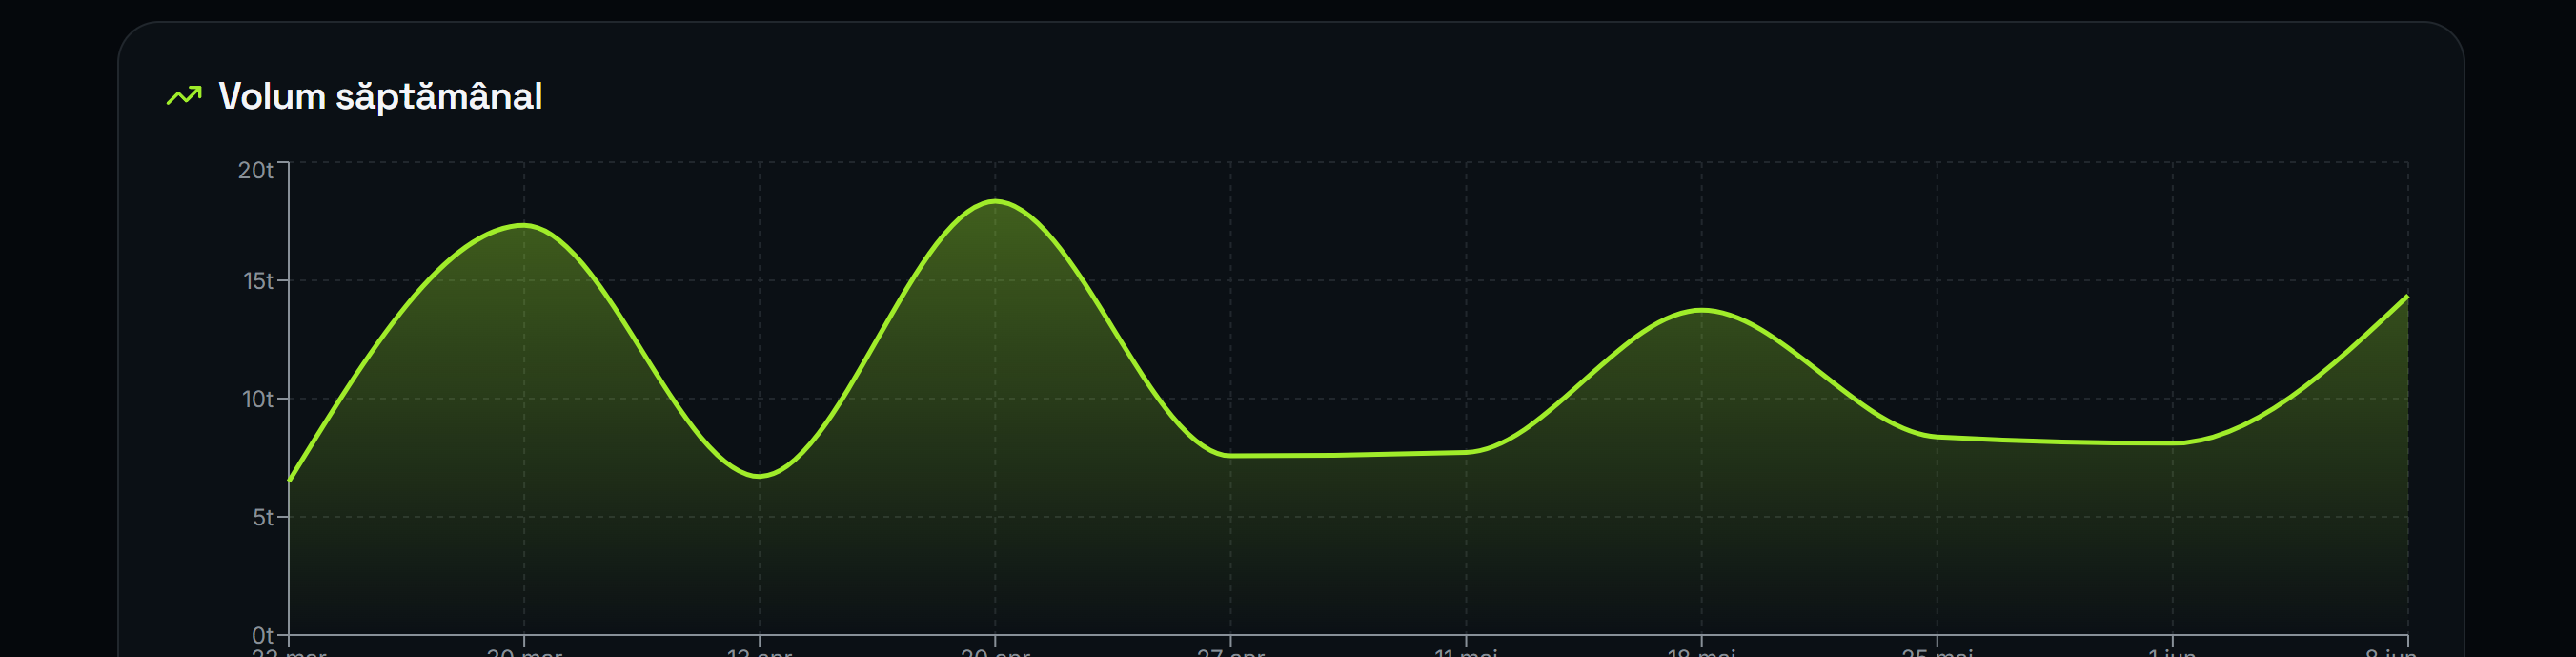
\includegraphics[width=\textwidth]{volume.png}
  \caption{Graficul volumului s\u apt\u am\^ anal}
  \label{fig:volume}
\end{figure}

\subsection{Predic\c tia 1RM \c si regresia liniar\u a}

Al doilea grafic (figura~\ref{fig:prediction}) aplic\u a regresia liniar\u a
peste valorile 1RM estimate de-a lungul timpului. Linia continu\u a reprezint\u a
valorile reale, cea punctat\u a tendin\c ta calculat\u a, iar por\c tiunea
final\u a proiecteaz\u a evolu\c tia probabil\u a pe urm\u atoarele patru
s\u apt\u am\^ ani.

\begin{figure}[H]
  \centering
  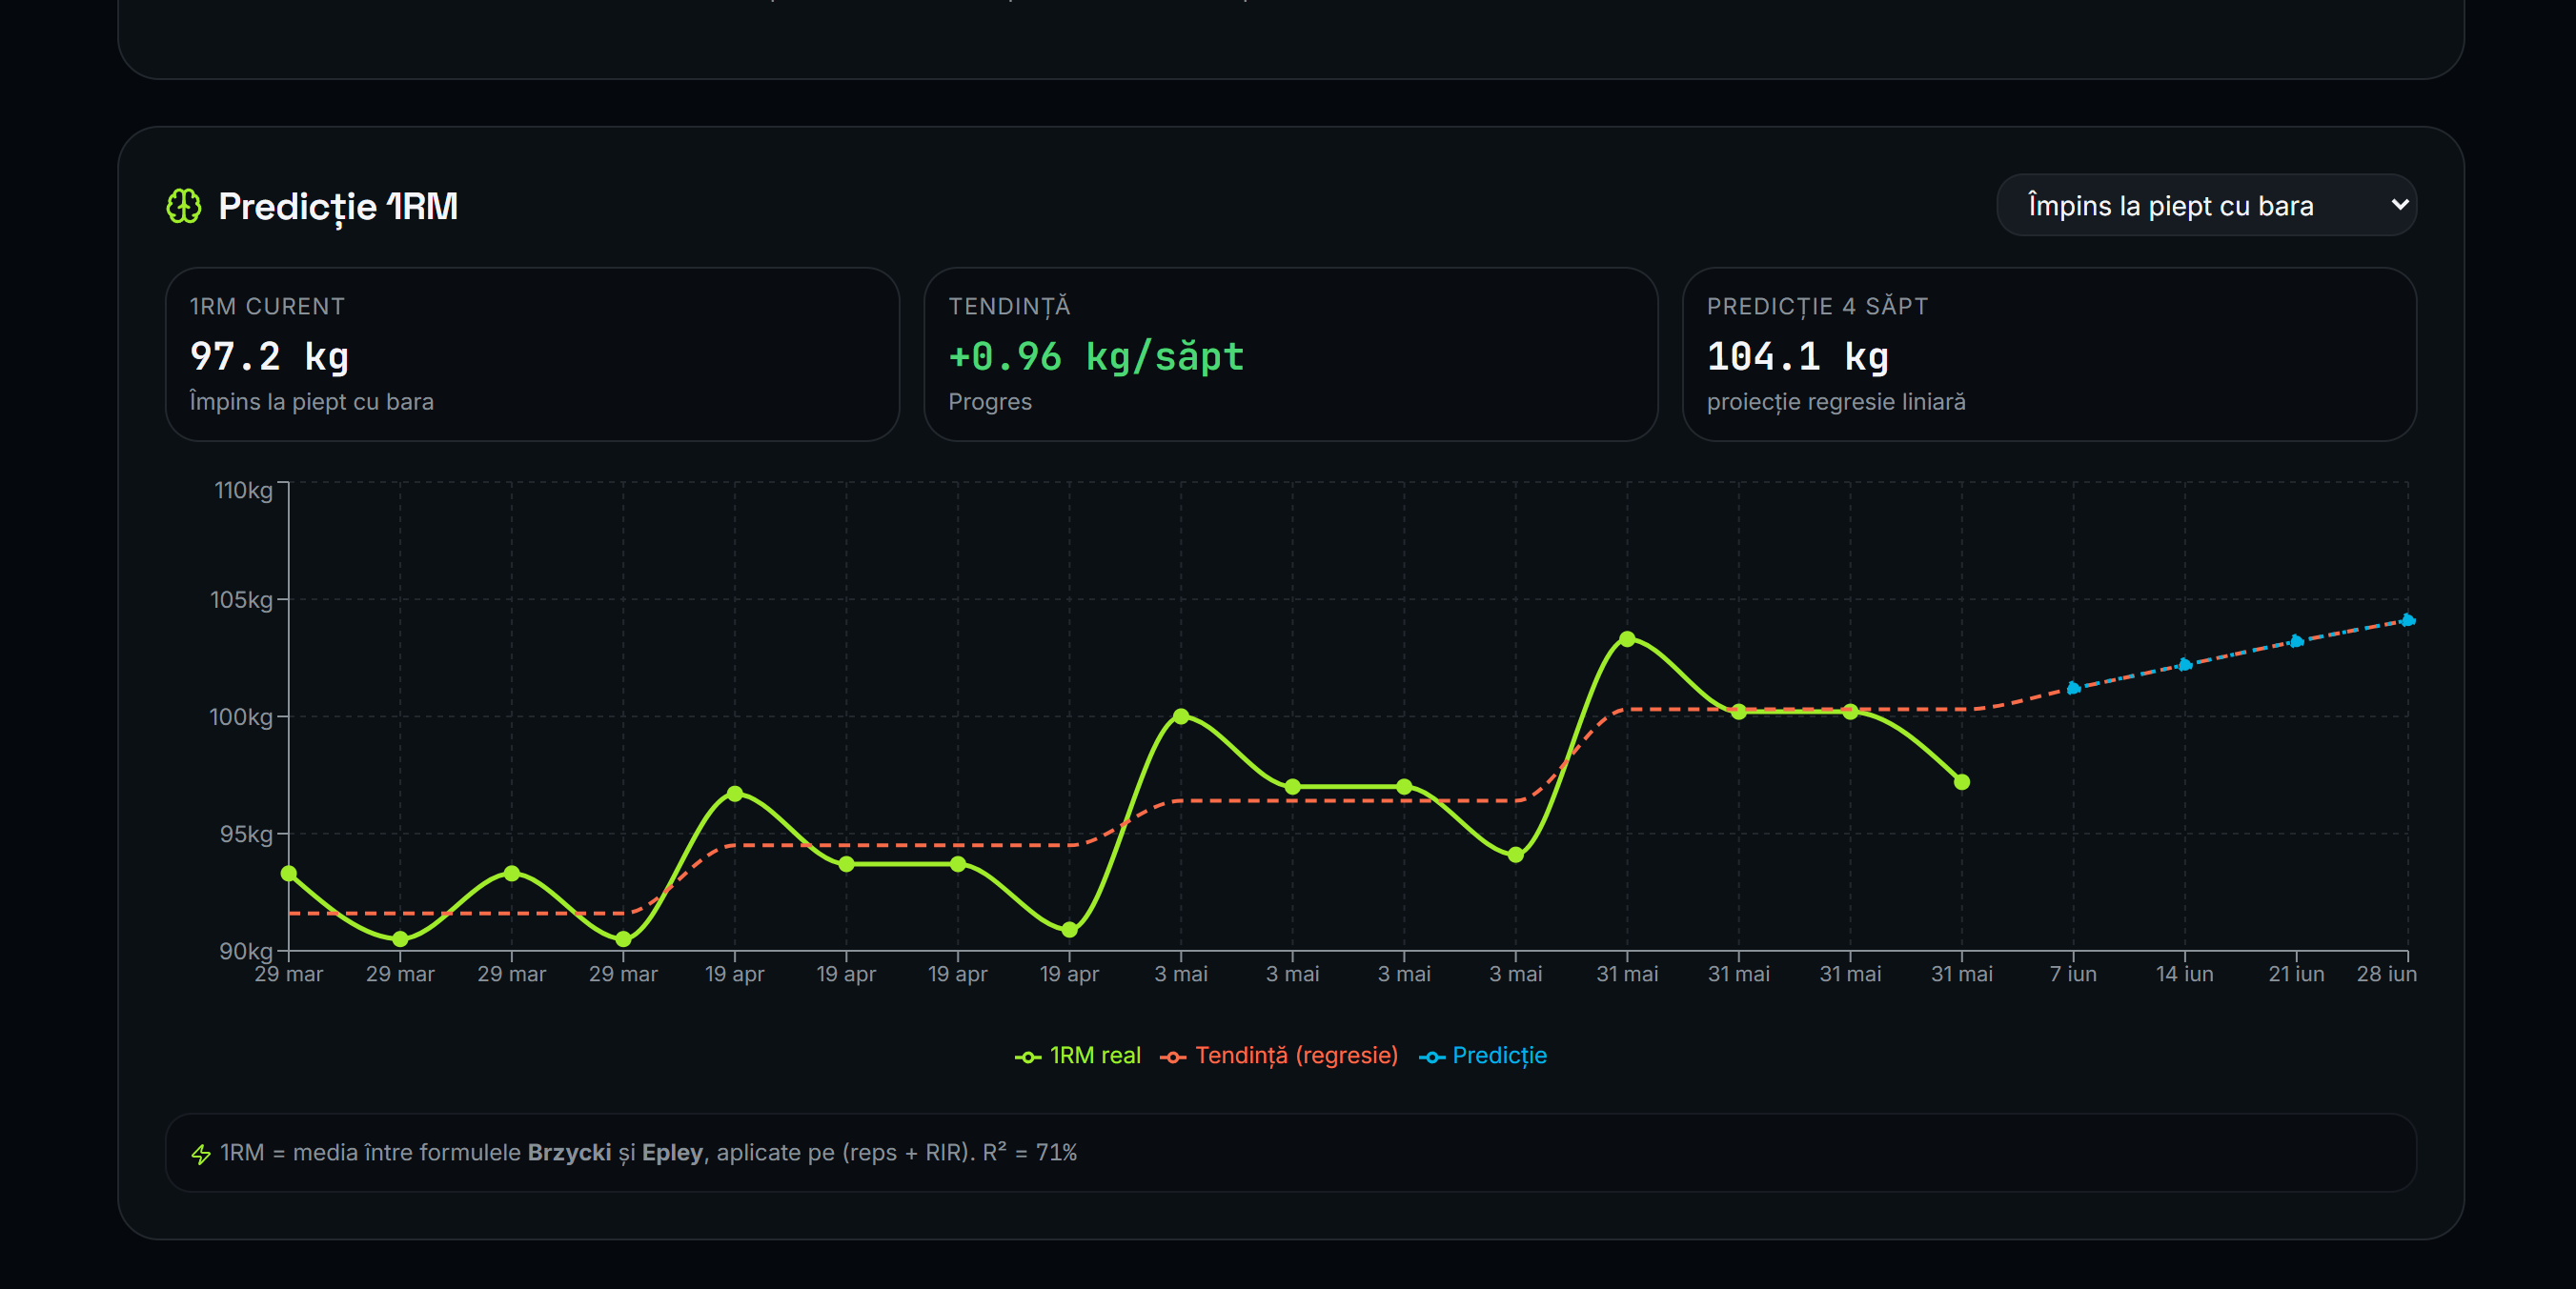
\includegraphics[width=\textwidth]{prediction.png}
  \caption{Predic\c tia 1RM \c si regresia liniar\u a}
  \label{fig:prediction}
\end{figure}

\subsection{Detec\c tia platourilor}

Atunci c\^ and volumul s\u apt\u am\^ anal scade cu peste 5\% pe parcursul a trei
s\u apt\u am\^ ani, aplica\c tia afi\c seaz\u a automat un avertisment de platou
(figura~\ref{fig:plateau}), suger\^ and utilizatorului c\u a ar putea avea
nevoie de o s\u apt\u am\^ an\u a de \textit{deload}. Astfel, stagnarea este
semnalat\u a \^ inainte s\u a devin\u a o problem\u a.

\begin{figure}[H]
  \centering
  
\includegraphics[width=\textwidth]{plateau.png}
  \caption{Detec\c tia platourilor}
  \label{fig:plateau}
\end{figure}
